\documentclass[a4, 12pt]{article}
\usepackage[paper=a4paper, top=2.5cm, left=2.5cm, right=2.5cm, bottom=2.5cm, headheight=1.0cm, headsep=1cm, footnotesep=0.5cm]{geometry}%
\clubpenalty = 10000
\widowpenalty = 10000
\usepackage[T1]{fontenc}
\usepackage{pslatex}%
\usepackage[utf8]{inputenc}
\usepackage{amsmath,amssymb}
\usepackage{bm}
\usepackage{tabularx}
\usepackage{graphicx}
\usepackage[english]{babel}
\usepackage{setspace}
\usepackage{url}

% \usepackage{natbib}
\usepackage[style=apa,
			backend=biber,
			maxcitenames=1,
			maxcitenames=2,
			uniquelist=true]{biblatex}
\DeclareLanguageMapping{english}{english-apa}
\addbibresource{literature.bib}

\usepackage{float}
% \usepackage{placeins}
\usepackage{lscape}
\usepackage{rotating}
\usepackage{multirow}
\usepackage{longtable}
\usepackage{booktabs,caption}
\usepackage{color}
\definecolor{red}{rgb}{1,0,0}

\usepackage{titlesec}
\usepackage{multicol}

\usepackage{array}
\usepackage{wrapfig}
\usepackage{colortbl}
\usepackage{pdflscape}
\usepackage{tabu}
\usepackage{threeparttable}
\usepackage{threeparttablex}
\usepackage[normalem]{ulem}
\usepackage{makecell}
\usepackage{xcolor}


\titleformat{\section}{\normalsize\bfseries}{\thesection}{1em}{}
\titleformat{\subsection}{\normalsize\bfseries}{\thesubsection}{1em}{}
\titleformat{\subsubsection}{\normalsize}{\thesubsubsection}{1em}{}

%CUSTOMISE LETTERING OF TITLE PAGE
% \makeatletter
% \renewcommand*{\@fnsymbol}[1]{\ensuremath{\ifcase#1\or *\or a  \else\@ctrerr\fi}}
% \makeatother

%TO ENABLE SUBSUBSECTION
\setcounter{secnumdepth}{3}
%TO SHOW SUBSUBSECTIONS IN TABLE OF CONTENTS
\setcounter{tocdepth}{3}

\usepackage{ifxetex,ifluatex}
\usepackage{fixltx2e} % provides \textsubscript
\ifnum 0\ifxetex 1\fi\ifluatex 1\fi=0 % if pdftex
  \usepackage[T1]{fontenc}
  \usepackage[utf8]{inputenc}
\else % if luatex or xelatex
  \ifxetex
    \usepackage{mathspec}
  \else
    \usepackage{fontspec}
  \fi
  \defaultfontfeatures{Ligatures=TeX,Scale=MatchLowercase}
\fi
% use upquote if available, for straight quotes in verbatim environments
\IfFileExists{upquote.sty}{\usepackage{upquote}}{}
% use microtype if available
\IfFileExists{microtype.sty}{%
\usepackage{microtype}
\UseMicrotypeSet[protrusion]{basicmath} % disable protrusion for tt fonts
}{}
\usepackage{hyperref}
\hypersetup{unicode=true,
            pdftitle={Untitled},
            pdfborder={0 0 0},
            breaklinks=true}
\urlstyle{same}  % don't use monospace font for urls
\usepackage{color}
\usepackage{fancyvrb}
\newcommand{\VerbBar}{|}
\newcommand{\VERB}{\Verb[commandchars=\\\{\}]}
\DefineVerbatimEnvironment{Highlighting}{Verbatim}{commandchars=\\\{\}}
% Add ',fontsize=\small' for more characters per line
\usepackage{framed}
\definecolor{shadecolor}{RGB}{248,248,248}
\newenvironment{Shaded}{\begin{snugshade}}{\end{snugshade}}
\newcommand{\KeywordTok}[1]{\textcolor[rgb]{0.13,0.29,0.53}{\textbf{#1}}}
\newcommand{\DataTypeTok}[1]{\textcolor[rgb]{0.13,0.29,0.53}{#1}}
\newcommand{\DecValTok}[1]{\textcolor[rgb]{0.00,0.00,0.81}{#1}}
\newcommand{\BaseNTok}[1]{\textcolor[rgb]{0.00,0.00,0.81}{#1}}
\newcommand{\FloatTok}[1]{\textcolor[rgb]{0.00,0.00,0.81}{#1}}
\newcommand{\ConstantTok}[1]{\textcolor[rgb]{0.00,0.00,0.00}{#1}}
\newcommand{\CharTok}[1]{\textcolor[rgb]{0.31,0.60,0.02}{#1}}
\newcommand{\SpecialCharTok}[1]{\textcolor[rgb]{0.00,0.00,0.00}{#1}}
\newcommand{\StringTok}[1]{\textcolor[rgb]{0.31,0.60,0.02}{#1}}
\newcommand{\VerbatimStringTok}[1]{\textcolor[rgb]{0.31,0.60,0.02}{#1}}
\newcommand{\SpecialStringTok}[1]{\textcolor[rgb]{0.31,0.60,0.02}{#1}}
\newcommand{\ImportTok}[1]{#1}
\newcommand{\CommentTok}[1]{\textcolor[rgb]{0.56,0.35,0.01}{\textit{#1}}}
\newcommand{\DocumentationTok}[1]{\textcolor[rgb]{0.56,0.35,0.01}{\textbf{\textit{#1}}}}
\newcommand{\AnnotationTok}[1]{\textcolor[rgb]{0.56,0.35,0.01}{\textbf{\textit{#1}}}}
\newcommand{\CommentVarTok}[1]{\textcolor[rgb]{0.56,0.35,0.01}{\textbf{\textit{#1}}}}
\newcommand{\OtherTok}[1]{\textcolor[rgb]{0.56,0.35,0.01}{#1}}
\newcommand{\FunctionTok}[1]{\textcolor[rgb]{0.00,0.00,0.00}{#1}}
\newcommand{\VariableTok}[1]{\textcolor[rgb]{0.00,0.00,0.00}{#1}}
\newcommand{\ControlFlowTok}[1]{\textcolor[rgb]{0.13,0.29,0.53}{\textbf{#1}}}
\newcommand{\OperatorTok}[1]{\textcolor[rgb]{0.81,0.36,0.00}{\textbf{#1}}}
\newcommand{\BuiltInTok}[1]{#1}
\newcommand{\ExtensionTok}[1]{#1}
\newcommand{\PreprocessorTok}[1]{\textcolor[rgb]{0.56,0.35,0.01}{\textit{#1}}}
\newcommand{\AttributeTok}[1]{\textcolor[rgb]{0.77,0.63,0.00}{#1}}
\newcommand{\RegionMarkerTok}[1]{#1}
\newcommand{\InformationTok}[1]{\textcolor[rgb]{0.56,0.35,0.01}{\textbf{\textit{#1}}}}
\newcommand{\WarningTok}[1]{\textcolor[rgb]{0.56,0.35,0.01}{\textbf{\textit{#1}}}}
\newcommand{\AlertTok}[1]{\textcolor[rgb]{0.94,0.16,0.16}{#1}}
\newcommand{\ErrorTok}[1]{\textcolor[rgb]{0.64,0.00,0.00}{\textbf{#1}}}
\newcommand{\NormalTok}[1]{#1}
\usepackage{graphicx,grffile}
\makeatletter
\def\maxwidth{\ifdim\Gin@nat@width>\linewidth\linewidth\else\Gin@nat@width\fi}
\def\maxheight{\ifdim\Gin@nat@height>\textheight\textheight\else\Gin@nat@height\fi}
\makeatother
% Scale images if necessary, so that they will not overflow the page
% margins by default, and it is still possible to overwrite the defaults
% using explicit options in \includegraphics[width, height, ...]{}
\setkeys{Gin}{width=\maxwidth,height=\maxheight,keepaspectratio}
\IfFileExists{parskip.sty}{%
\usepackage{parskip}
}{% else
\setlength{\parindent}{0pt}
\setlength{\parskip}{6pt plus 2pt minus 1pt}
}
\setlength{\emergencystretch}{3em}  % prevent overfull lines
\providecommand{\tightlist}{%
  \setlength{\itemsep}{0pt}\setlength{\parskip}{0pt}}
% Redefines (sub)paragraphs to behave more like sections
\ifx\paragraph\undefined\else
\let\oldparagraph\paragraph
\renewcommand{\paragraph}[1]{\oldparagraph{#1}\mbox{}}
\fi
\ifx\subparagraph\undefined\else
\let\oldsubparagraph\subparagraph
\renewcommand{\subparagraph}[1]{\oldsubparagraph{#1}\mbox{}}
\fi

%%% Use protect on footnotes to avoid problems with footnotes in titles
\let\rmarkdownfootnote\footnote%
\def\footnote{\protect\rmarkdownfootnote}

\begin{document}
\begin{titlepage}
% Titlepage (fold)
\thispagestyle{empty}%
\begin{center}
\renewcommand{\baselinestretch}{1.0}\normalsize %
\textbf{
The effect of music education on students' well-being. Empirical evidence from a field experiment}\\[1cm]
Preliminary - work in progress \\[1cm]
This draft: \today \\[1cm]
% Comments welcome \\[0.25cm]
% \renewcommand{\baselinestretch}{1.5}\normalsize
Vera Schramm \\
University of Halle-Wittenberg \\[0.75cm]
% \today
 \end{center}


\end{titlepage}

\renewcommand{\baselinestretch}{1}\normalsize

\textbf{\normalsize Abstract}
Our analyses, following the discussion above, address two central questions
using a cultural capital framework. First, who participates in music
both in and outside of school, and to what extent is such involvement
stratified by social class, race/ethnic, and gender status? Second, and relative
to the more central question discussed at the outset, do various forms of
music involvement influence academic achievement, even after accounting
for prior achievement, background statuses, and other educationally meaningful
investments? Relatedly, to what extent might disparities in music
involvement shape group-specific gaps in achievement that have been so well
documented elsewhere?

\clearpage
\tableofcontents

\clearpage
\doublespacing
\pagestyle{plain}

\hypertarget{introduction}{%
\section{Introduction}\label{introduction}}

\label{sec:introduction}

In German schools, and music are often considered less important than the typical hard subjects like math and science. Due to a lack of teachers, many classes are cancelled, of which 80\% are in the subject of music. In Saxony we see ongoing efforts to eliminate the subject of music from the curriculum entirely. Furthermore, the quality of music lessons suffers from the fact that 80\% of its teaching staff are foreign to the subject (Möller, 2017).

Music education experts are concerned about this development. According to them, music should not be regarded as a private matter. Regardless of their socioeconomic background, school children must have the opportunity to receive high level music education because it is as important for a proper education as literacy and mathematics (Gebert, 2018). Prof.~Höppner, the General Secretary of the German Music Council (Generalsekretär des Deutschen Musikrats), said in an interview that music education helps to build stable self-esteem by learning to access ones own emotions (Stoverock, n.d.). He points out that the phase where music can shape a young person explicitly well is completed by the age of 13. That stresses the importance of high quality music education for students in pre- and secondary school.

The Federal Association of Music Education (Bundesverband Musikunterricht (BMU)) has set up the ``Agenda 2030'' to initiate an improvement in music education. Similar to Höppner (Stoverock, n.d.), they consider music education as valuable and essential for a social and cultural society. It encourages children to take responsibility and to increase their sense of self-determination (Bundesverband Musikunterricht (BMU), 2016, p. 2).

In views of this broad societal debate, empirical research has concentrated on the effect of music education on cognitive abilities (school grades and IQ in particular). Not so much effort was spent on observing the connection of music and well-being. This seems surprising because life satisfaction and happiness have become central research areas in the social sciences. My thesis addresses this research gap and investigates the effects of music education on children's overall life satisfaction and on satisfaction in specific areas, namely satisfaction with the class, satisfaction with friends, and satisfaction with the situation at school. It analyzes music education in the classroom where fifth and sixth grade students have one additional hour of music education per week. The project is called ``klasse.im.puls'' and it promotes the establishment of musical training in secondary schools in Bavaria. The program was implemented with the intention to give every child the opportunity to learn how to play an instrument. Additional positive outcomes were expected: an increase in self-confidence and social competence, as well as a reduction in violent behavior.\footnote{For more information:} The project was supervised by the FAU Erlangen-Nuremberg Music Teaching Departement in collaboration with the Bavarian Ministry of Education.
My analysis focuses on the change in the overall life satisfaction and in satisfaction within specific areas reported by the students over the course of the project. The term of \emph{life satisfaction} refers to a cognitive evaluation of a person's reaction to his or her life in contrast to \emph{affect}, an ongoing emotional reaction. Combined, LS and affect yield subjective well-being (Diener, 2009, p. 71). I will approach the problem by using a multi level model, that accounts for differences on the level of the individual student, on the level of the class and on the school level. I do this by using Bayesian inference\ldots{}

The interest in life satisfaction as an outcome of the music project stems from the idea that higher values of LS come with many benefits. Among other positive correlates, adolescents reporting very high levels of LS are less likely to be affected by depression, anxiety, negative affect and social stress compared to adolescents with very low life satisfaction. Also, they achieve higher SEAs and demonstrate higher mean scores of school satisfaction (Gilman \& Huebner, 2006, p. 316; Proctor, Linley, \& Maltby, 2009, p. 928). These results go in line with a study by Suldo \& Huebner (2004, p. 94) that shows that LS could be a moderating variable in predictions of the development of psycho-pathological behaviors. Low life satisfaction may be an indication for externalizing behavior problems in the future. When life satisfaction is on a higher level, those behavior problems are less likely to occur (Suldo \& Huebner, 2004, p. 100) The authors conclude that life satisfaction might operate as a buffer against the development of subsequent externalizing behavior problems ``in the face of stressful life events'' (Suldo \& Huebner, 2004. p.~101). Kim, Conger, Elder, \& Lorenz (2003) add to the discussion that externalizing behavior problems in turn lead to more stressful life events. That reciprocal interrelation of stressful life events and externalizing problems (reported as delinquent behaviors) leads to unhealthy dynamics of increasing stress and behavior problems. If higher LS leads better coping mechanisms with stressful life events, these dependencies could be reduced.
LS is also positively correlated with children having higher measures of self-esteem, internal locus of control, and extraversion (Huebner, 1991a, p. 107). These features help in building a solid foundation for later life. On the other hand, dissatisfaction with life is associated with adolescents having poor mental health (like anxiety and neuroticism) and physical health and being exposed to a higher risk of considering or attempting suicide (Huebner, 1991a, p. 107; Valois, Zullig, Huebner, \& Drane, 2004, p. 94). Furthermore, Zullig, Valois, Huebner, Oeltmann, \& Drane (2001, pp. 284--185) show that adolescents reporting low levels of overall life satisfaction are more likely to use drugs and alcohol earlier in life and in higher amounts than adolescents with medium or high life satisfaction.

Considering the statement of Höppner, one would expect the project to positively effect students' life satisfaction. Evidence for this relation would lend credibility to the project and support its continuation. It could also stress the importance of music education and signal the Ministry of Culture to keep music education in the curriculum and work on its implementation in federal states alongside Bavaria. However, there will be no in-depth investigation of the analysis of any observations. Describing possible reasons for certain outcomes must be left to music and education experts\ldots{}

The structure of my thesis is as follows: At first there will be an overview of the current literature on music effecting students' lives. Next, the project and the dataset will be explained. Descriptive statistics are presented alongside a detailed diagnostic on pre-treatment differences in the treatment group compared to the control group. The estimation strategy is presented in chapter four, following the results in the fifth chapter. Finally, chapter six concludes and discusses.

\emph{Gute Einleitung bei Southgate \& Roscigno (2009)}

\hypertarget{music}{%
\section{Music}\label{music}}

\clearpage

\label{sec:literature_review}
With regard to the effect of music on students' lives, most of the researchers are interested in academic outcomes and intelligence among students who are actively involved in music. Generally, there is the predominant perception of a positive link between music and cognitive abilities. Osborne, McPherson, Faulkner, Davidson, \& Barrett (2015, p. 14) observed improved math skills and higher subjective well-being scores in children that were part of a music project. He also found them to have a better self-control over impulsive behavior. Yang (2015) (p.~385),Wetter, Koerner, \& Schwaninger (2008) (p.~372) , Hille (2014) (p.~62), and Guhn, Emerson, \& Gouzouasis (2019) (p.~316) present evidence that children playing music have better grades at school. But this conclusion is not very meaningful as all of these studies follow a correlational design and do not allow for causal inference. Nonetheless, the very optimistic and as we will see not quite realistic belief has prevailed that playing music causes children to achieve better results at school. This conclusion needs to be \emph{revised}. In an extensive review of the available evidence concerning associations between music and cognitive abilities, the picture is not so clear any longer (Schellenberg \& Weiss, 2013). Small associations between music training and mathematical ability in correlational and quasi-experimental studies might result from individual differences in general intellectual ability (p.~527). The available evidence simply indicates that high-functioning children (i.e., higher IQ, better performance in school) are more likely than other children to take music lessons and to perform well in mathematics and other tests of cognitive ability (p.~534). This fits with the Hille (2014) study where the outcome difference in cognitive skills between musically active and inactive children reduces greatly when holding constant observable characteristics. An other plausible interpretation of study outcomes that fail to detect a causal relationship comes from Wetter et al. (2008). He points out the possibility that the relationship is explained by affluent parents being more likely to afford music lessons for their child and thus, the socio-economic background may be the cause of higher performance at school. Despite the weakness of the above studies to draw causal inference, there is slight evidence that there may be a causal direction \emph{from} music training \emph{to} cognitive abilities in a study by Schellenberg (2004). He compares two treatment groups who receive piano lesson and voice lesson respectively to a control group in which the children have drama lessons. Random assignment to the different conditions allowed for inference that music lessons caused small increases in cognitive abilities (namely larger increases in full-scale IQ). However, this does not preclude the possibility that high-functioning children are more likely driven to play music. The misconception of music being a predictor for academic achievement is also discussed by Southgate \& Roscigno (2009) (p.~17) who states that music is rather a mediator, to some degree, of family background and student status. Results from a meta-analysis, suggest that music training does not reliably enhance children and young adolescents' cognitive or academic skills, and that previous positive findings were probably due to confounding variables, such as placebo effects and lack of random allocation of participants (Sala \& Gobet, 2016, p. 64). The effect size was reduced in studies that applied a proper study design (random allocation of participants to the treatment group and comparison to an active control group). With respect to the mathematical outcomes, the only study comparing a music training to an active control group and with random allocation of the participants to the group (Mehr, Schachner, Katz, \& Spelke, 2013) found a negative effect size. These considerations are in clear contrast to the popular perception that music training enhances any non-music related cognitive skill.

However positive outcomes due to music could be found outside academics. The Norwegian psychologist and musicologist Even Ruud who in 1978 was the head of the first music therapy training performed extensive studies on music and identity. He states that cultural activities, explicitly music, can ``contribute to a feeling of quality of life and the subjective sense of health.'' (p.~96). In an experimental study by Costa-Giomi (2004) a positive causal effect was detected of piano lessons on self-esteem {[}144{]} but she did not find an effect on math computation scores. One especially popular project that was conducted to improve children's lives is Venezuela's National Music Education Program ``El Sistema''. It is a large scale social music education program established by José Abreu in the 1970s. 300,000 children are equipped with instruments every year and receive regular after-school lessons and are playing in orchestras. The initial goal was to prevent children from using drugs and being involved in violence and crime which was successfully achieved. Being in orchestras also enhanced social behavior of the students through greater concern for others and their own well-being (Uy, 2012, p. 13). However positive effects go far beyond keeping adolescents away from drugs and violence: El sistema teaches the participating students to ``reflect and act upon the world in order to transform it'' {[}7{]}. Playing in an orchestra means joy, motivation, teamwork, the aspiration to success {[}6{]}. The students pick up management and organizational skills and responsibility due to many roles and rules that they need to follow to sty in the program{[}p.~10{]}. Also, being in an orchestra gives the students the change to conceptualize themselves as part of something much larger and greater (p.~11) and they learn to express greater concern for others' and their well being (p.~13). El Sistema became internationally popular and was replicated in several countries. Osborne et al. (2015) reviewed the outcome of El Sistema inspired projects in Australia and found significantly higher subjective well-being scores in the participating group (p.~14). Students from the music program also had better self-control over impulsive behavior (p.~15). However, other studies come to contrary conclusions and fail to show a significant effect of music participation on well-being, social skills, emotional intelligence or self-esteem (Portowitz, Lichtenstein, Egorova, \& Brand, 2009, p. 121; Schellenberg, 2011, p. 190 association). Again, findings are diffuse and therefore interpretation of any results needs to be with caution.

The takeaway from this section is we must be very careful when drawing causal conclusion and we have to adjust the methods.

This paper complements existing literature by using different music indicators and estimation strategies to provide further insight on the relationship between music and education as well as the potential sources of endogeneity.

\clearpage

\hypertarget{data}{%
\section{Data}\label{data}}

\label{sec:data}
\#\# Pre-treatment differences

\hypertarget{the-project}{%
\subsection{The project}\label{the-project}}

\label{project}
The data come from the years 2012-2014 when KIP was conducted in six different secondary schools (Mittel- und Realschulen) in Nuremberg. Generally, there are different types of implementations of the KIP project (e.g.~choir, brass band, string orchestra) among which the rock band model was implemented in all of the schools that are subject to this study. Probably due to parents' and students' music preferences, this type has been the most popular. A school was able to apply for the project if certain criteria were fulfilled. For example, the school had to make sure that there was a full-time music teacher who was qualified to carry out the project. That person was trained to lead a band class and attended yearly meetings with other music teachers to share experiences. This way, it can be assured that the treatment in each school looked pretty much the same and there were no noteworthy differences in the way the teachers arranged the music lessons in the band classes. Participating schools were supported in acquiring equipment and instruments to implement ensemble music class teaching. In each school was a band class and a control class. The band classes received three music lessons per week, whereas the control classes only received two lessons of regular music education. Music lessons in the treatment classes differed significantly from that in the control group. In the band classes, the teachers had a more practical approach and there was less theoretical music education than in the control group. The three music lessons per week were split into a) Instrumental instructions in small groups, b) ensemble playing, and c) general music education (music theory or history). The latter was similar to how regular music education was implemented in the control group. Thefor not only the amount of music education is higher in the treatment group but also the way that music education is delivered differs a lot from normal music lessons in a way that it is more practical and with better equipment. The students played concerts in regular intervals and were thus able to share what they had learned. In five different points of time, the students were asked to fill in a questionnaire:

wave 1: Beginning of 5th grade (pre-treatment)
wave 2: Mid of 5th grade
wave 3: end of 5th grade
wave 4: mid of 6th grade
wave 6: end of 6th grade

In total, 394 students were observed, however not all of them occur in each wave. Some questions were only asked in wave 1 (i.e.~sex) which leads to the problem that there were no information about gender for students who did not attend in the first wave. Only 309 reported their gender in wave 1 which leads to 85 students for whom the gender is ``unknown''. To not miss all of these observations in regressions including gender, NAs were replaced by a category ``unknown''. The same was done for the variable of migration background and language spoken at home. An other issue to point out is the comparably low number of observations in wave 5 in school 5.

Students had to rate their level of life satisfaction on a scale reaching from 0 (``completely unsatisfied) to 10 (completely satisfied) for the question''How satisfied are you with your life overall?"

\hypertarget{selection-process-and-pre-treatment-differences}{%
\subsection{selection process (and pre-treatment differences)}\label{selection-process-and-pre-treatment-differences}}

The decision who attended the treatment group was made before the entrance to grade 5. Parents could choose to put their child into a music class. Therefore, the experiment is not fully randomized. Children who were already into music in the first place might have been more likely to have chosen the music class. Also the decision can be a a consequence of parental and socio-economic background of the student. To have a better idea of possible differences between the treatment and the control group, I computed standardized mean differences:

The standardized mean differences are not a reason of concern in this setting. For most of the observed variables, there are no notable differences between the treatment group and the control group. However, as already suspected, there are differences in prior musical knowledge. Among the treated, there are relatively more children who have music as a hobby before the project has even started. Of the 87 students who answered with ``yes'' to the question if music was their hobby, only 24 were assigned to the control group and the remaining 63 students attended the band classes. Also, the duration of making music is very different in the two subgroups. In the Treatment group, 56\% are parcticing at leats 30 min, while in the control group that share is only 35\%. However, the model addresses this issue by applying a difference-in difference approach to estimate the causal effect of additional music lessons on students' well-being. accounts for the individual musical background of the child by. Therfore the fact that the model accounts for musical background of the student, differences in the control group and the treatment group are not a problem for inference.

\hypertarget{measuring-ls-in-children}{%
\subsection{Measuring LS in children}\label{measuring-ls-in-children}}

An extensive amount of research was done on adult life satisfaction and on methods how to measure it. From that we know that not only is life satisfaction a result of life circumstances but it determines outcomes in several areas like health, \ldots{} (see Firsch 1999 for a review (suldo and huebner, ß. 94))

Even though, the amount of research on
\label{measurement}
To investigate ones quality of life, research uses both objective and subjective indicators. Typical objective indicators are the income levels, crime rates, and access to medical services -- measures that are external and quantifiable. Subjective indicators on the other hand comprise subjective evaluations of ones' individual life circumstances (Gilman \& Huebner, 2000, p. 178). Only a modest relation between both measures was found which indicates that each approach carries uniqe information that are relevant for a comprehensive understanding of overall life quality \emph{(Veenhofen, 1996)}. Over time, measurement methods for subjective indicators have evolved leading to substantial growth in the life satisfaction research. However, for a long time, most of the measurements were designed to assess adults' life satisfaction. Only recently, investigating correlates of life satisfaction in adolescents has begun. One reason why life satisfaction research in children was put off for a long time are probably that measuring life satisfaction in children is more challenging than for adults. Instruments for assessing children's subjective life satisfaction reports have been less intensively developed which is probably due to the fact that a Likert-type ratings scale is more difficult to use for younger children than for adolescents (Chambers \& Johnston, 2002, p. 28). For example, younger children or children with poorer readings skills are less able to respond appropriately to negative items on questionnaires and this effect biases the interpretation of children's responses (Marsh, 1986, p. 45). It is also common for children rating their subjective life satisfaction to show elevated extreme scores. As children become older, this tendency shriks and they are more capable of providing graded ratings in between the two extremes. These results have potentially substantial implications for the interpretation of self-report ratings form children \emph{this tendency might have an erroneous and invalid impact on the interpretation of children's self-reports}(Chambers \& Johnston, 2002, pp. 33--34). When dealing with self-reported life satisfaction in children, it is crucial that the respective child fully understands the question in order to give a valid response (Gluskie, 2012; Tomyn, Fuller-Tyszkiewicz, Cummins, \& Norrish, 2016). One must make sure that a child is old enough to know how to use a satisfaction scale. This requires children to distnace themselves from the current situation, cognitively evaluate their life satisfaction (considering all relevant areas of life) and rate the degree to which certain items on the scale apply to them. This requires abstract thinking, which children develop in early adolescent years (10-14 years) (Gluskie, 2012; Piaget, 1955, 1969). Gilman \& Huebner (2000) have reviewed five different (both unidimensional and multidimensional) measurements explicitly developed to asses adolescents' life satisfaction.\footnote{The Students' Life Satisfaction Scale (Huebner, 1991b), the Satisfaction With Life Scale (Diener, Emmons, Larsen, \& Griffin, 1985), the Perceived Life Satisfaction Scale (Adelman, Taylor, \& Nelson, 1989), the Comprehensive Quality of Life Scale - School Version (Cummins, 1997; Gullone \& Cummins, 1999), and the Multidimensional Student's Life Satisfaction Scale (Huebner, 1994)} The authors evaluated those measures in terms of validity and reliability and found all of the scales to be appropriate for research with adolescents {[}181-188{]}. The demographic characteristics of the available samples show that all of the adolescents observed were older than 12 years. Therefor it remains unclear if children younger than that age are able to report valid satisfaction.
An other instrument was developed more recently by (Cummins \& Lau, 2005) which is the Personal Well-being Index (PWI-SC). Again, studies demonstrated reliability for this instrument as well (Casas \& Rees, 2015; Casas et al., 2011; Tomyn \& Cummins, 2011; Tomyn, Stokes, Cummins, \& Dias, 2019). But also in those studies, all of the adolescents were at least 12 years of age, mostly even older. There is only very little evidence on the psychometric properties of the PWI-SC for children below the age of 12.
One of them is González-Carrasco, Casas, Malo, Viñas, \& Dinisman (2016, p. 70) who applied the instrument for children as young as only 9 years and also found adequate fit of the data.
On the other hand, Tomyn et al. (2016) conducted a study with children aged 10-12 and concluded that subjective well-being data of children must be interpreted with caution. They also show that response bias towards the extreme positive end of a scale is higher with decreasing age. The authors do not recommend using the PWI-SC for children younger than 12 years. As for the specific sample, the PWI-SC did not serve as a valid instrument for measuring the SWB.

In conclusion, measuring life satisfaction in children is more challenging than for adults and is still in progress. It is advisable to check the validity and reliability of their data when testing children. Considering, the majority of the children from the KIP project are 10 year sold in wave 1 (72\% of those participating in wave 1), they might be just too young to give valid responses when asked about their life satisfaction. This must be kept in mind when evaluating the significance of the results.

\hypertarget{descriptive-statistics}{%
\subsection{Descriptive statistics}\label{descriptive-statistics}}

\label{descriptives}

\clearpage

\hypertarget{econometrics}{%
\section{Econometrics}\label{econometrics}}

\label{sec:econometrics}
Andrew Gelman (2013) consider a multilevel model to be ``a regression (a linear or a generalized linear model) in which the parameters - the regression coefficients - are given a probability model'' (p.~1). Mcelreath (2020) (p.~14) suggests to think of parameters as a placeholder for a missing model. That probability model itself has parameters called hyperparameters which are also estimated from the data. In other words, they are parameters for parameters. Their priors are often referred to as hyperpriors. Technically, there is no limit to the number of levels, however infeasable computation and ability to understand the model are in practice a restriction. The structure of my data is a hierarchical one as discussed in the \ref{sec:data}. Usually, in that case a simple nonhierarchical model is inappropriate. It tends to underfit when there are only few parameters and to overfit the data when too many parameters are included. This leads to models that fit the existing data well but lead to poor predictions for new data (Andrew Gelman (2013), 101). In the following, I will explain how hierarchical models are best to navigate between underfitting and overfitting (fit to sample always - not true of multilevel models - improves as we add parameters. Though multilevel models are more complicated, it is worth using them because they reduce overfit as new parameters are added (Youtube Video MacElreath Lecture 7). Hierarchical structure reduces overfit.

\hypertarget{identification}{%
\subsection{Identification}\label{identification}}

\label{sec:identification}
Bayesian inference starts with a prior distribution on the unknown parameters and updates this with the likelihood of the data, yielding a posterior distribution which is used for inferences and predictions (gelman and hill p143)
Kennedy (p.2) points out that with Bayesian methods it is important for Bayesian methods to pass through two phases: pre-experiment prophylaxis and post-data model evaluation, criticism, and extension. I will follow this documenting the process of finding appropriate priors and critically assessing the posterior distribution after running the model.

To assess the effect of the music treatment on the student's life satisfaction, the model must be able to identify causal inference. This would be a comparison between the observed life satisfaction in each student in the treatment group and that student's outcome were he participating in the treatment. Multilevel modeling works well for drawing causal inference but also for prediction and descriptive modeling (Andrew Gelman, 2013, p. 6). Multilevel models are especially useful for studying effects that vary by group. To study this variation among groups with classical regression, you need interactions. Using interactions has the disadvantage that estimates can be very noisy, in particular when there are only few observations in one group. Related to this is the problem of estimating group-level quantity with classical estimation. Again, small sample size in the group leads to useless information. On the other hand, ignoring group-level variation can also be misleading. Multilevel models can be a solution for the issue because the account for similarities between groups but also see that there are differences. The way they do that is by partially pooling information across units in the data in order to produce better estimates for all units. In this case, all the data are used to perform inference fr groups with small sample size instead of just using local information. Partial pooling can be seen as a compromise between the two extremes discussed above: Running separate regressions on each group level on one hand and completely ignoring variation between groups. This is referred to as no-pooling and complete pooling respectively. Both approaches can be useful as preliminary estimates, leading up to the partial pooling that comes out of a multilevel analysis. Therefore I will illustrate both the complete pooling and the no-pooling approach to compare them to partial pooling. To do so, I use simulated data.

\begin{itemize}
\item
  Underfitting: The model is insensitive to the details in the data. Learning too little from it.
\item
  Overfitting: The model is sensitive to the details in the data. Learning too much from it.
\item
  Multilevel models, also sometimes referred to as hierarchical models, involve predictors at different levels of variation. For example, in studying the treatment outcome of the KIP project, I have information about individual students (Age, sex, grades etc.), school-level information and time trends. Though the school level information are unobserved, as well as the time trends, it is important to account for effects on these levels. A multilevel model in this contexts allows to include effects that very by group (school) and time. It is very well possible that the intervention is more effective in some schools than others. This outcome would help to identify why this afterwards. An other helpful feature of multilevel modeling is that it allows one to estimate to the extend supported by the data and not being limited to the number of observation per school (which is the case for the no-pooling method.)
  After all, schools are different but they are also similar in the way that each school helps to estimate the treatment effect in other schools. I aim for a multilevel model, which simultaneously estimatesan intercept for each school and the variation among schools (macelreath p 416).
  Bayesian inference appropriate for multilevel modeling - natural to fit probability distributions to batches of parameters (gelman and hill p 143)
\end{itemize}

When the dynamics of mean life satisfaction for each school are plotted individually (\ref Figure), it is clear that some bias would enter the analysis if I ran only a single regression.

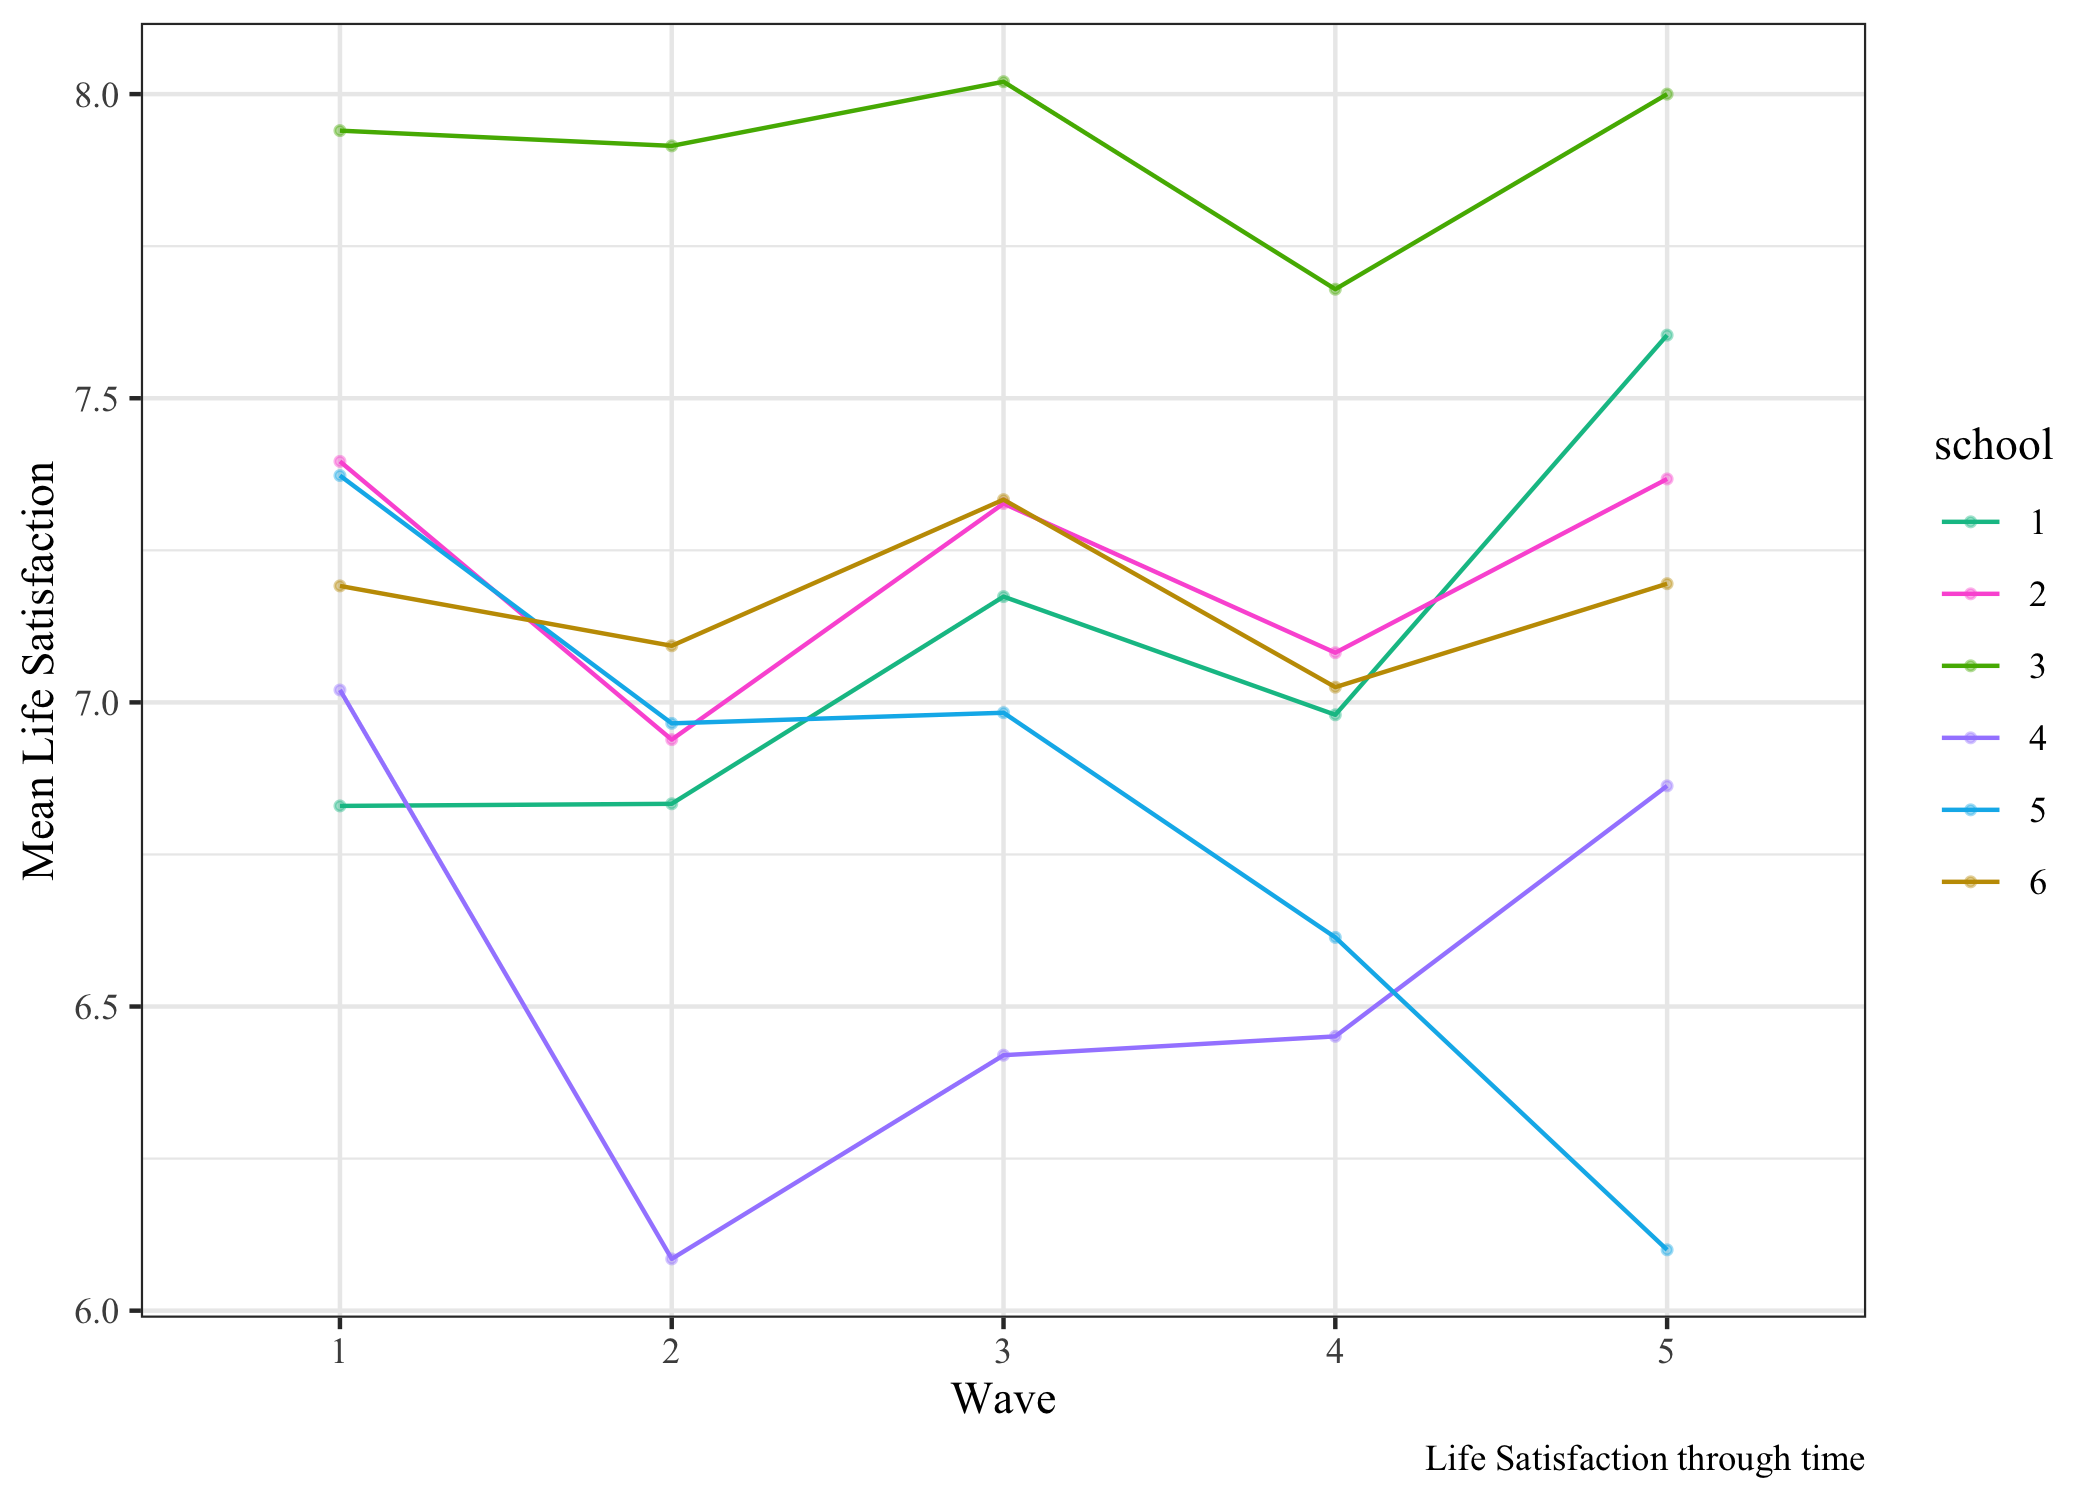
\includegraphics[width=1\linewidth]{../figures/lsat_vs_time_by_school}
Also, standard deviations are very big for the estimates as we will see in the no-pooling method, which suggests that some borrowing of strength through multilevel model may be appropriate.

\begin{itemize}
\item
  We want the regular features of the sample! Chapter 7 MacElreath
\item
  Strategie: One way: Regularizing priors. They are skepitcal of impossible relationships. They regularize inference. Regularizing force. Better predictions. / Cross-validation compares / Information criteria. Regularizing priors. Prior predictive simulation. Choose priors that will only creaty possible outcomes. Helps to reduce overfitting.
\item
  Complete pooling: This means the population of schools is assumed to be invariant. If clusters are ignored, which means to assign the same intercept to each of them, then there is the risk of ignoring important variation in how schools correspond to the treatment. This variation could mask association with other variables (Mcelreath, 2020, p. 416)
\item
  No-pooling: This means that each school can tell nothing about any other school as if variation among schools were assumed to be infinite.
\item
  Partial pooling: This means using an adaptive regularizing prior that prevents the model from ``getting too excited by the training sample'' (Mcelreath, 2020, p. 218). A regularizing prior is a prior that slows down the rate of learning from a sample and thus reduces overfitting while still allowing the model to learn the regular features of a sample. Resulting from regularization is a phenomenon sometimes called shrinkage \ldots{} (Mcelreath (2020), p.~419) Estimates for each cluster are less underfit than the grand mean and less overfit than the no-pooling estimates. The partial pooling produces noticeably better estimates when there are only a few observations in one group. In that case, the no pooling estimate well be especially overfit. Otherwise, the varying effect estimates are not that different from the no pooling estimates. The partial pooling tends to improve estimates about each cluster. This improved estimation leads to several, more pragmatic sounding, benefits of the multilevel approach:
\end{itemize}

\begin{enumerate}
\def\labelenumi{\arabic{enumi}.}
\tightlist
\item
  Improved estimates for repeat sampling
\item
  Improved estimates for imbalance in sampling
\item
  Estimates of variation
\item
  Avoid averaging, retain variation
\end{enumerate}

\hypertarget{complete-pooling}{%
\subsection{Complete pooling}\label{complete-pooling}}

\begin{table}[H]

\caption{(\#tab:complete pooling)Estimates complete pooling}
\centering
\begin{tabu} to \linewidth {>{\raggedleft}X>{\raggedleft}X>{\raggedleft}X>{\raggedleft}X}
\toprule
wave & complete & lower & upper\\
\midrule
1 & -0.0171144 & -0.3985530 & 0.3643241\\
2 & -0.1543548 & -0.5153323 & 0.2066226\\
3 & 0.3483488 & -0.0247137 & 0.7214114\\
4 & -0.3285619 & -0.7027461 & 0.0456223\\
\bottomrule
\end{tabu}
\end{table}

\hypertarget{no-pooling}{%
\subsection{No-pooling}\label{no-pooling}}

\begin{table}[H]

\caption{\label{tab:no-pooling}Estimates no-pooling}
\centering
\begin{tabu} to \linewidth {>{\raggedleft}X>{\raggedleft}X>{\raggedleft}X>{\raggedleft}X>{\raggedleft}X}
\toprule
school & wave & estimate & lower & upper\\
\midrule
1 & 1 & -0.2126153 & -0.5037749 & 0.0785443\\
1 & 2 & -0.2338833 & -0.5205275 & 0.0527609\\
1 & 3 & -0.1318997 & -0.4227986 & 0.1589992\\
1 & 4 & -0.1845208 & -0.4722545 & 0.1032128\\
2 & 1 & -0.1625532 & -0.6963053 & 0.3711989\\
\addlinespace
2 & 2 & -0.1838212 & -0.7130579 & 0.3454154\\
2 & 3 & -0.0818376 & -0.6153290 & 0.4516537\\
2 & 4 & -0.1344587 & -0.6647848 & 0.3958674\\
3 & 1 & 0.4478898 & -0.0819770 & 0.9777565\\
3 & 2 & 0.4266218 & -0.0987296 & 0.9519731\\
\addlinespace
3 & 3 & 0.5286054 & -0.0010007 & 1.0582114\\
3 & 4 & 0.4759843 & -0.0504565 & 1.0024250\\
4 & 1 & -0.7582930 & -1.2949003 & -0.2216857\\
4 & 2 & -0.7795610 & -1.3116529 & -0.2474691\\
4 & 3 & -0.6775774 & -1.2139240 & -0.1412308\\
\addlinespace
4 & 4 & -0.7301985 & -1.2633798 & -0.1970171\\
5 & 1 & -0.5744479 & -1.1097624 & -0.0391334\\
5 & 2 & -0.5957159 & -1.1265150 & -0.0649168\\
5 & 3 & -0.4937323 & -1.0287861 & 0.0413215\\
5 & 4 & -0.5463534 & -1.0782419 & -0.0144648\\
\addlinespace
6 & 1 & -0.7582930 & -1.2907278 & -0.2258581\\
6 & 2 & -0.7795610 & -1.3074804 & -0.2516415\\
6 & 3 & -0.6775774 & -1.2097515 & -0.1454033\\
6 & 4 & -0.7301985 & -1.2592074 & -0.2011896\\
\bottomrule
\end{tabu}
\end{table}

\hypertarget{estimation}{%
\subsection{Estimation}\label{estimation}}

\hypertarget{the-model}{%
\subsubsection{The model}\label{the-model}}

\label{estimation}
(Gelman p13)
In a first step, I will set up a full probability mode - a joint probability distribution for all observable and unobservable quantities in a problem. The model should be consistent with knowledge about the underlying scientific problem and the data collection process.
After that I will calculate and interpret the appropriate posterior distribution - the conditional probability distribution of the unobserved quantities of ultimate interest, given the observed data.
Finally, in a third step the fit of the model will be evaluated and the models' implications of the resulting posterior distribution is presented (how sensitive are the results to the modeling assumptions in step 1?)

We have repeat measures and heterogeneity across clusters (McElreath). After all, schools are different but each school does help estimating the treatment effect in other schools.
The study of effectiveness of the music project, with the students in school \(j\) having a certain unknown parameter vector \(\theta_j\), it might be reasonable to expect that estimates \(\theta_j\), which represent a sample of schools, should be related to each other. This is achieved in a natural way by using a prior distribution in which life satisfaction is viewed as a sample from a common \emph{population distribution}. A key feature of such applications is that the observed data, \(y_{ij}\), with student index \(i\) within group indexed by \(j\), can be used to estimate aspects of the population distribution of the \(theta_j\)'s even though the values of \(\theta_j\) are not themselves observed. In contrast, hierarchical models can have enough parameters to fit the model well, while using a population distribution to structure some dependence into the parameters, thereby avoiding problems of overfitting.

I simultaneously investigate the treatment in six different schools. The analysis is restricted to wave 1 (pre treatment) and wave 2 (post treatment). The regression equation is:

The hierarchical structure in my model looks as follows:
\[lsat \sim {\sf Normal} (\mu_{ijt}, \sigma),\]
\[\mu_{ijt} = \beta_0 + \beta_{1j[i]} T_i + \sum\limits_{l=2}^5\delta_{lj[i]} (T_{i} \times \text{Period}_{t}) + \lambda_t + \mu_{j[i]} + \alpha_{i} + \epsilon_{ijt},\]
\[\beta_0 \sim  {\sf Normal}(7,2),\]
\[Population-level effects \sim {\sf Normal}(0,5),\]
\[Group-level effects \sim {\sf Cauchy}(0,1),\]
\[\sigma \sim {\sf Exponential}(0,5)\]

where

\begin{itemize}
\tightlist
\item
  \(y_{ijt}\) is the outcome of pupil \(i\) in school \(j\) at time \(t\).
\item
  \(T_{i}\) is a binary indicator of whether or not pupil \(i\) is in the treatment group. We model a fixed effect for the treatment group because the treatment takes place at the aggregate level (class). Therefore, bias in the estimate of the treatment effect may results from unobserved factors at the class level.
\item
  \(\delta_{l2j[i]}\) is the treatment effect in wave \(l\). The effect is allowed to vary across schools.
\item
  \(\lambda_t\) denotes period fixed effects.
\item
  \(\alpha_{i}\) models individual-specific unobserved factors. Individual heterogeneity is model because we have repeated observations for the same pupils over time.
\item
  \(\epsilon_{it}\) is an error term.
\end{itemize}

(Simulation?)

For doing \emph{blah} I use \emph{blub} {[}ref{]}

\hypertarget{prior-distribution}{%
\subsubsection{Prior distribution}\label{prior-distribution}}

As stated above in \ref(section\ldots{} parameters are not point estimates but they have distributions in a Bayesian framework. The specification for these parameters are called prior distribution because they must be specified before the model is fit to data and it assigns them a probability to every possible value of each parameter to be estimated. If the specification is done properly, for all parameters in the model, a Bayesian model yields a joint prior distribution on parameters and data, and hence a prior marginal distribution for the data (Gabry p5). This process can be described as the prior distributions and data interacting to finally produce the posterior distribution. The posterior can be seen as a compromise between the prior distribution and the likelihood function. Therefore, the choice of the prior should be done carefully since it can determine the outcome severely. After identifying the type of data being described, creating a descriptive model with meaningful parameters, and defining a likelihood function, the next step is to establish a prior distribution over the parameter values (kruschke 110). The prior distribution indicates the believes about the distribution of each parameter without knowing the specific data. Depending on the choice of prior and the respective data set, the ``compromise'' favors one them over the other. Flat priors or super-vague priors (\(\sf {N}(0,1e6)\)) are usually not recommended. They lead to a posterior distribution that is mainly influenced by the data which means that though the data set is very well described by the model but predictions are very poor. The model only ``learned'' about the distribution from the data because the prior did not carry any information. However if the prior has strong believes about the distribution of the parameters, meaning the prior distribution is sharply peaked, and there are only relatively few data, the posterior distribution is more influenced by the prior. Generally, weakly informative priors (\(\sf{N}(0,10)\)) are recommended because they help by providing a very gentle nudge towards reasonable values of the parameter (mcelreath p 299). If there is a reasonable large amount of data, they will dominate while the prior becomes less important. In case of not very meaningful data though, the ``weakly informative prior'' make up for it by strongly influencing the posterior inference. This relation is illustrated in figure \ref{}. The upper row shows the posterior that appears when having a prior distribution \(lsat \sim {\sf Normal}(5, 200)\). The standard deviation in this prior is huge an gives barely any useful information about the distribution of life satisfaction among the population. The shape of the posterior is almost identical to the one of the likelihood. The opposite is the case when the prior is highly informative. A normal distribution with parameters of \(\mu = 5\) and \(\sigma = 1\) suggests that life satisfaction is very narrow around the mean of 5. The prior is so sharp that the posterior distribution is noticeably influenced by the prior. Bayesian models with proper priors are generative models (Gabry p5)

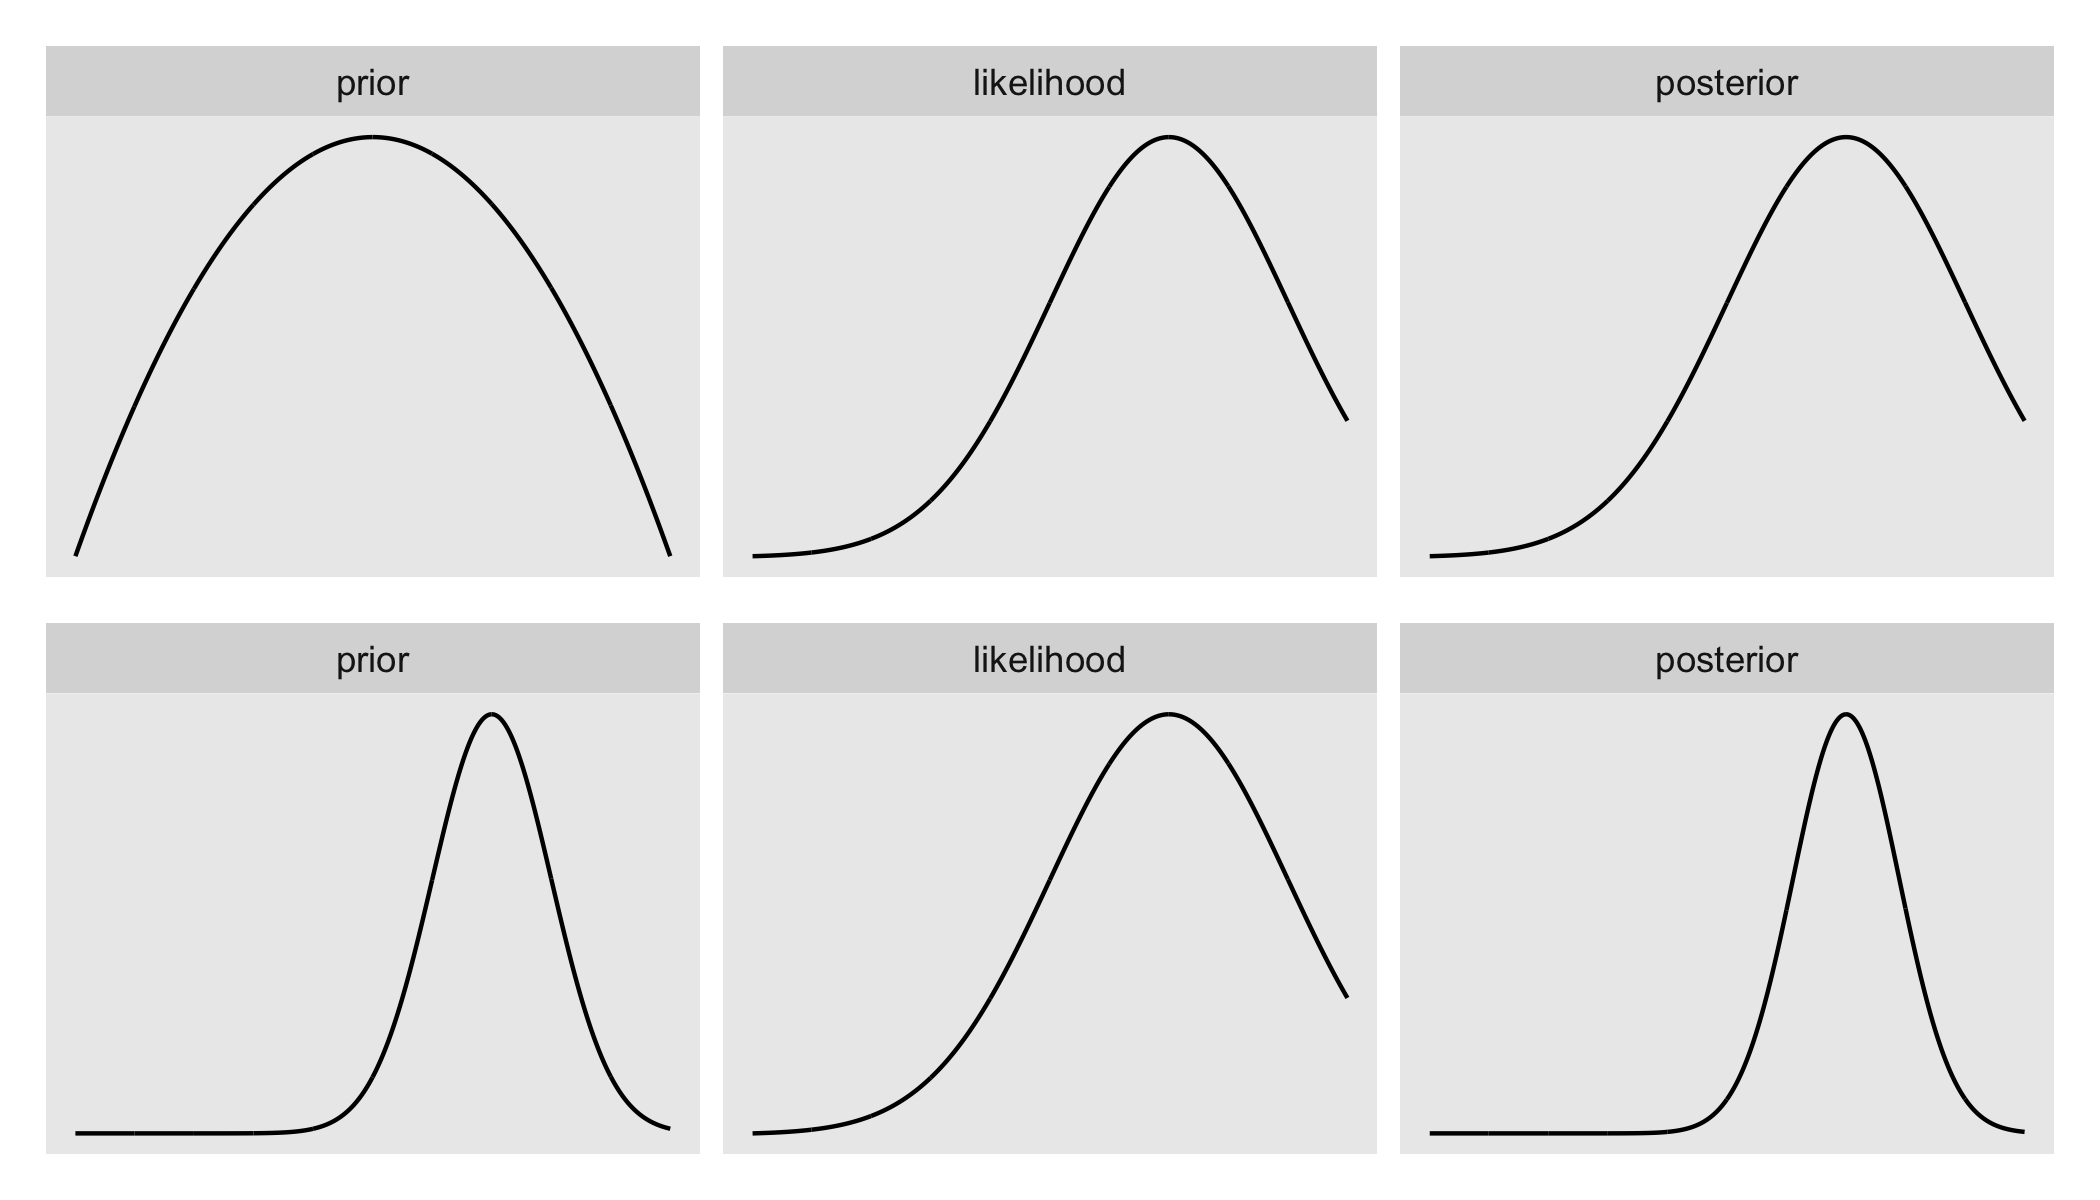
\includegraphics[width=1\linewidth]{../figures/flat_peaked}
To decide on proper priors, I made some prior predictive simulations as suggested by MacElreath. This method is useful for understanding the implication of a prior and is neatly executed by Gabry ( see full code\ldots). It simulates predictions from a model, using only the prior distribution instead of the posterior distribution. Once priors are chosen, they imply a joint prior distribution of individual life satisfaction (elreath p85). This procedure is based on choosing priors conditional on pre-data knowledge of the data, on general facts so to say (elreath, p100). Only when this step is done, the model is applied to the data.

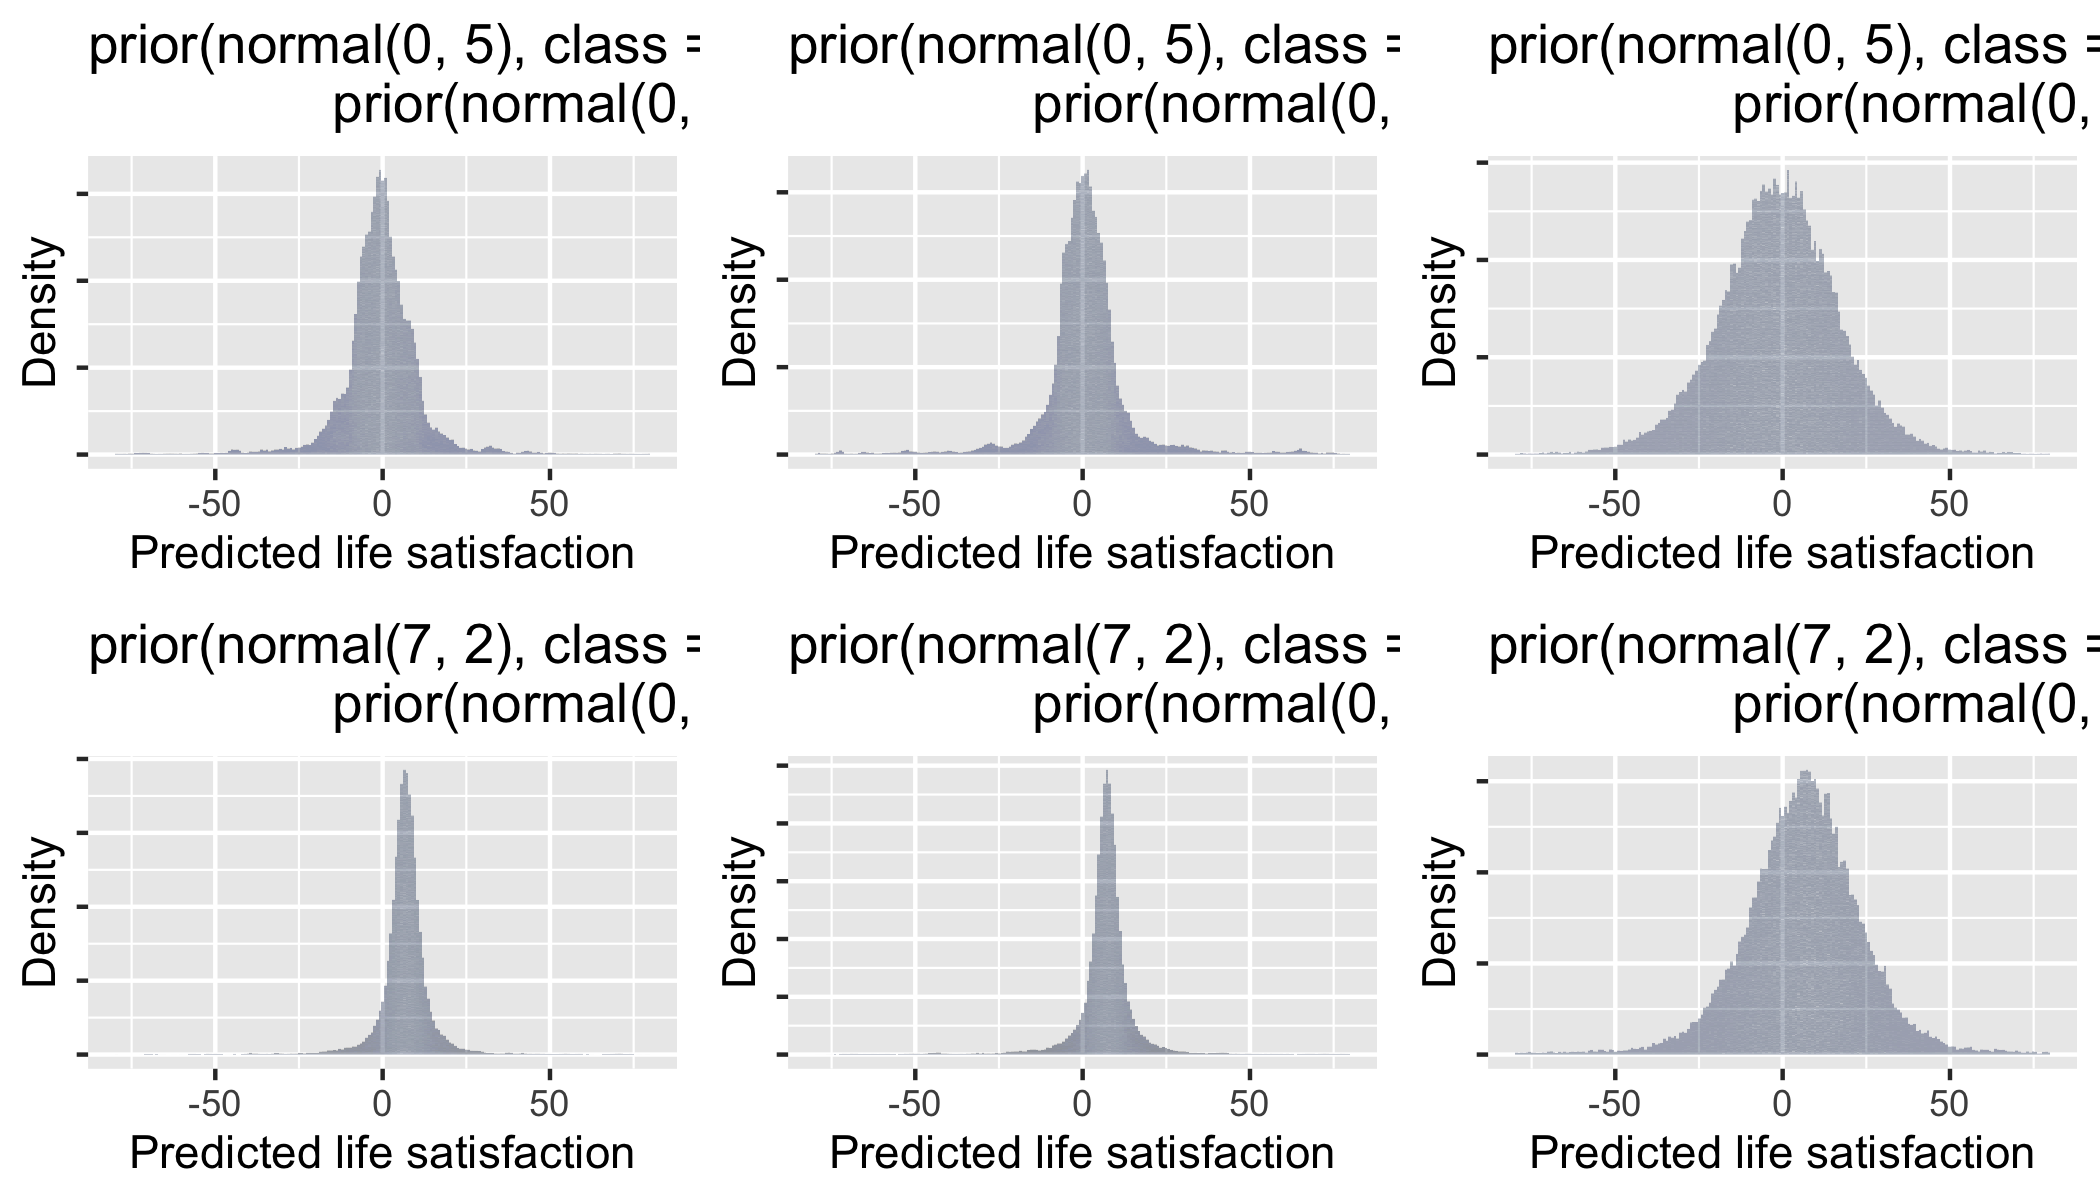
\includegraphics[width=1\linewidth]{../figures/lsat_predicted}

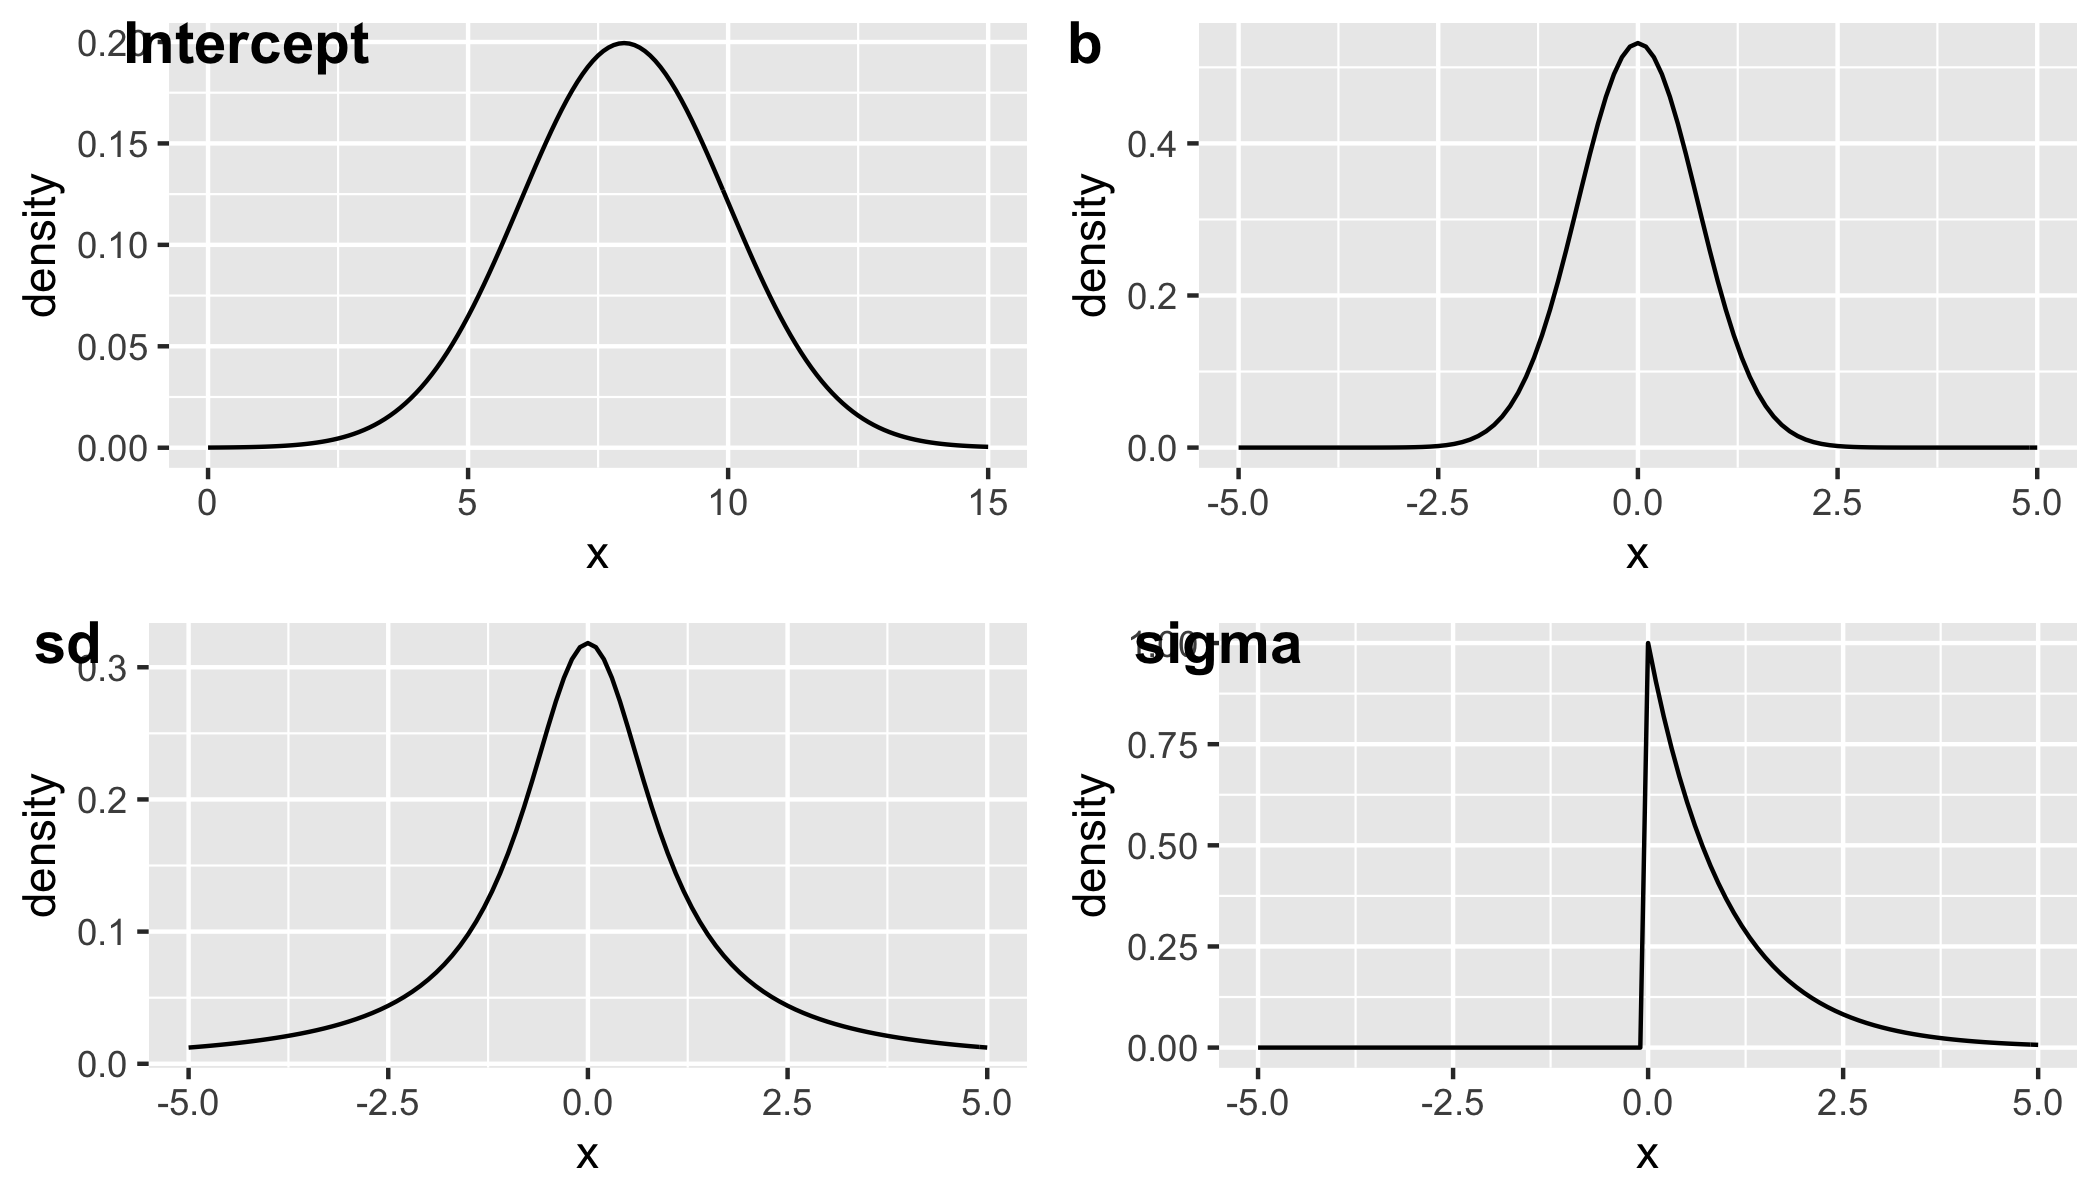
\includegraphics[width=1\linewidth]{../figures/chosen_priors}

\clearpage

\hypertarget{results}{%
\section{Results}\label{results}}

\label{sec:results}

As described in Section 4, estimation biases resulting from selection into treatment take place at two stages: The initial decision to take up music lessons and the decision not to give up until age 17\ldots{} At such a young age, the choice of a long-term extracurricular activity such as music is strongly determined by the parents. For the parents, however, we observe a large number of characteristics, in particular their socio-economic status, personality, involvement with the child's education, and taste for the arts\ldots{} (Hille, 2014, p. 65)
NOTE: I have to observe parents (``parental background differences'')
NOTE: Results in Hille (2014) might be driven by unobserved heterogeneity\ldots{} unobserved individual characteristics could still determine the decision to keep on playing music until age 17 rather than giving up earlier (p.~67).
NOTE: Sensitivity of Hille (2014) results to reverse causality by performing mediation analysis in which we estimate the correlation between music practice and outcome p, while subsequently controlling for all outcomes q rather than p (p.~67). How do I address the issue of reverse causality?
Three challenges should determine the agenda of future research on this agenda.
1. separate the influence of parental and individual background from that of music (identify a variable that increases the likelihood to learn a musical instrument without affecting the development of skills.)
2. answer the question of the extent to which extracurricular activities are substitutable (substitutes vs.~compliments).
3. long-term effects of music training on outcomes such a s labor market success or life satisfaction

\hypertarget{partial-pooling}{%
\subsection{Partial pooling}\label{partial-pooling}}

\begin{table}[H]

\caption{(\#tab:partial pooling)Estimates partial pooling}
\centering
\begin{tabu} to \linewidth {>{\raggedleft}X>{\raggedleft}X>{\raggedleft}X>{\raggedleft}X>{\raggedleft}X}
\toprule
school & wave & mean & Q10 & Q90\\
\midrule
7 & 1 & 0.1806651 & -0.3164921 & 0.6909753\\
7 & 2 & -0.2062209 & -0.6898667 & 0.2894317\\
7 & 3 & 0.3448464 & -0.1488093 & 0.8530004\\
7 & 4 & -0.3541457 & -0.9917535 & 0.2854370\\
\bottomrule
\end{tabu}
\end{table}

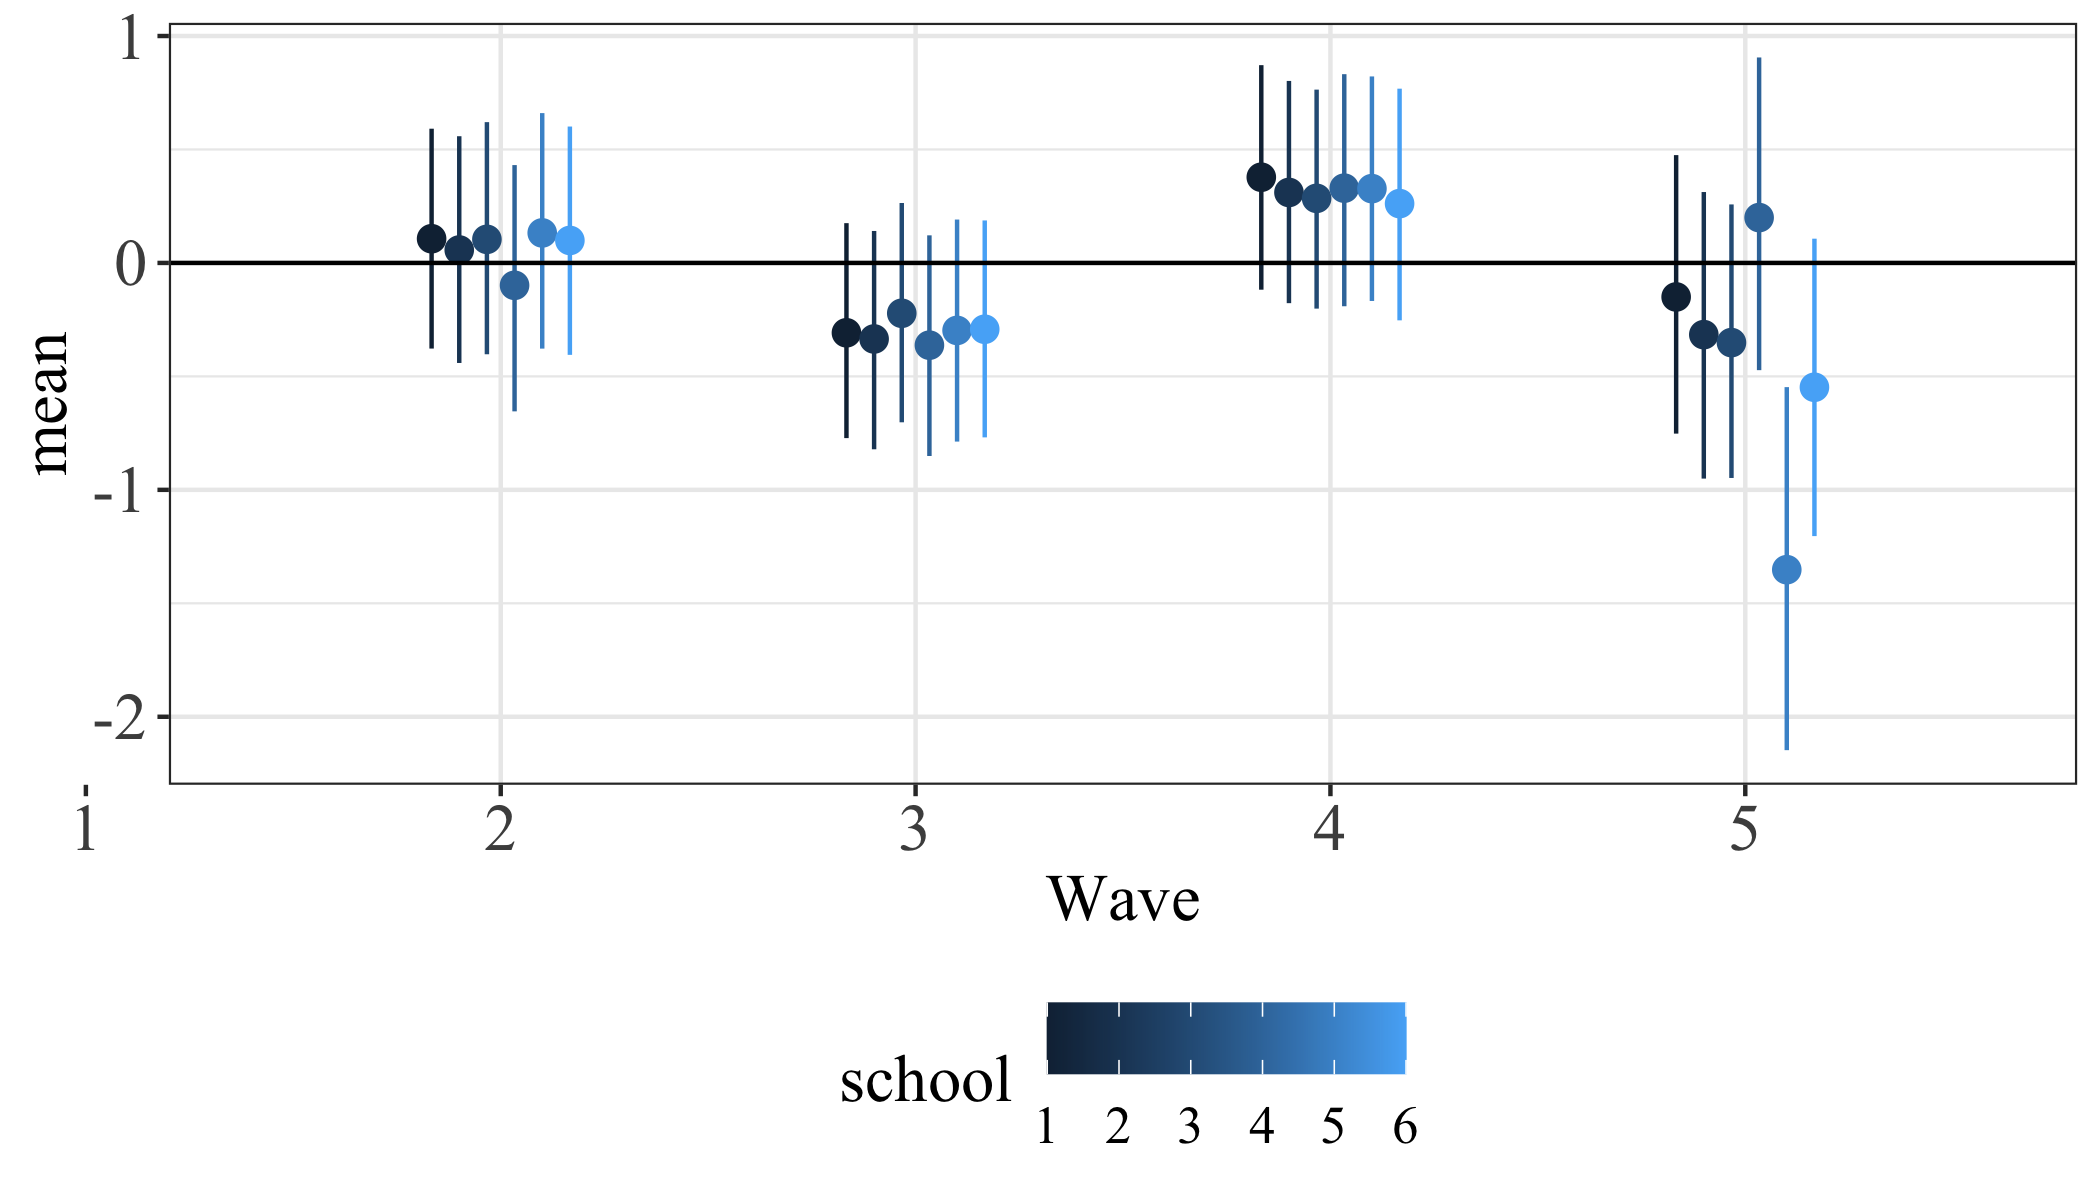
\includegraphics[width=1\linewidth]{../figures/lsat_teff_across_schools}

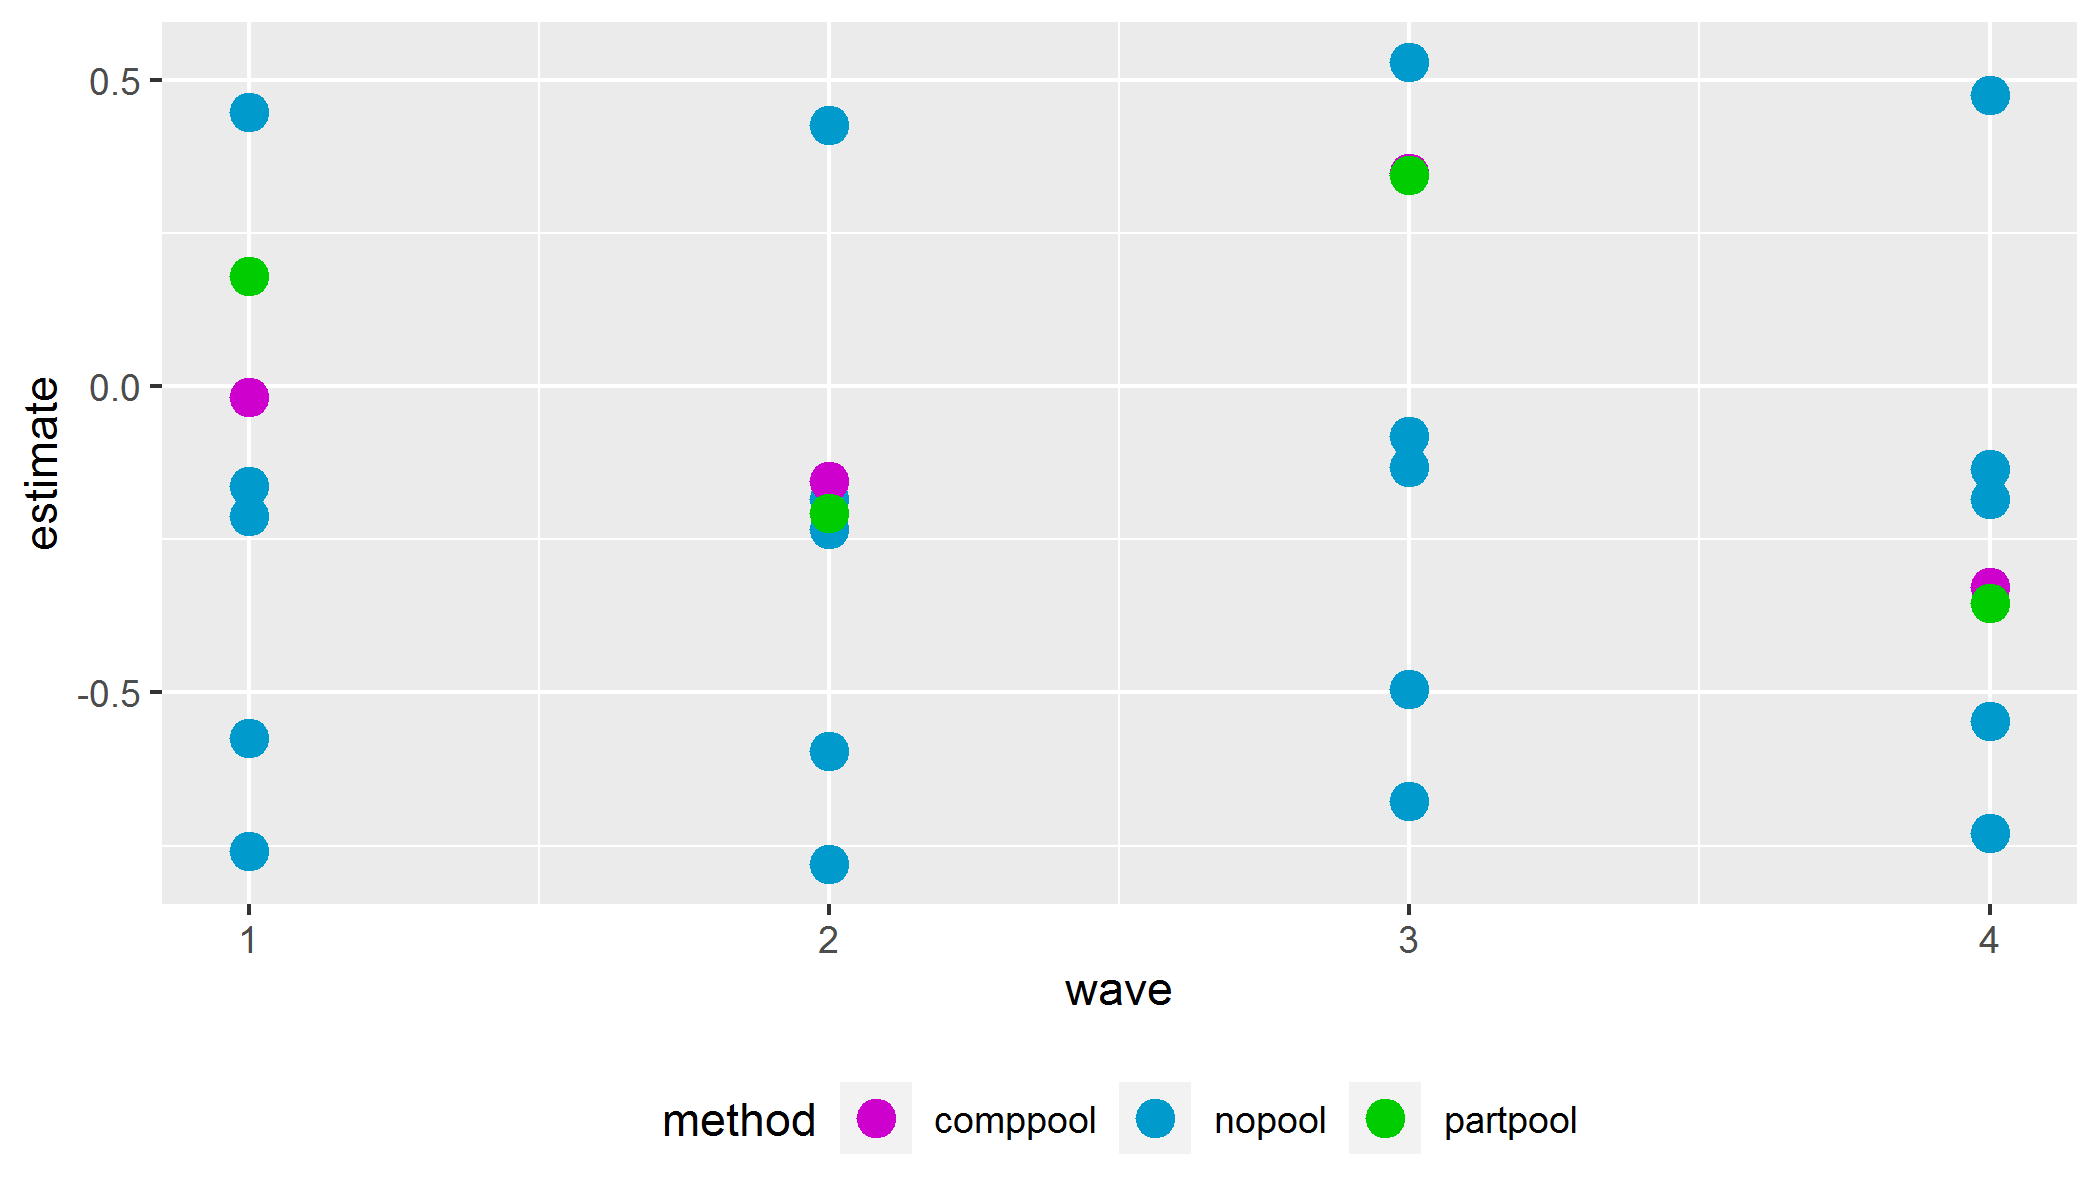
\includegraphics[width=1\linewidth]{../figures/compare_estimates_lsat}

\begin{table}[H]

\caption{(\#tab:compare methods)Estimates generated by different methods}
\centering
\begin{tabu} to \linewidth {>{\raggedleft}X>{\raggedleft}X>{\raggedleft}X>{\raggedleft}X>{\raggedleft}X>{\raggedleft}X>{\raggedleft}X>{\raggedright}X}
\toprule
school & wave & estimate & lower & upper & Q10 & Q90 & method\\
\midrule
1 & 1 & -0.2126153 & -0.5037749 & 0.0785443 & NA & NA & nopool\\
1 & 2 & -0.2338833 & -0.5205275 & 0.0527609 & NA & NA & nopool\\
1 & 3 & -0.1318997 & -0.4227986 & 0.1589992 & NA & NA & nopool\\
1 & 4 & -0.1845208 & -0.4722545 & 0.1032128 & NA & NA & nopool\\
2 & 1 & -0.1625532 & -0.6963053 & 0.3711989 & NA & NA & nopool\\
\addlinespace
2 & 2 & -0.1838212 & -0.7130579 & 0.3454154 & NA & NA & nopool\\
2 & 3 & -0.0818376 & -0.6153290 & 0.4516537 & NA & NA & nopool\\
2 & 4 & -0.1344587 & -0.6647848 & 0.3958674 & NA & NA & nopool\\
3 & 1 & 0.4478898 & -0.0819770 & 0.9777565 & NA & NA & nopool\\
3 & 2 & 0.4266218 & -0.0987296 & 0.9519731 & NA & NA & nopool\\
\addlinespace
3 & 3 & 0.5286054 & -0.0010007 & 1.0582114 & NA & NA & nopool\\
3 & 4 & 0.4759843 & -0.0504565 & 1.0024250 & NA & NA & nopool\\
4 & 1 & -0.7582930 & -1.2949003 & -0.2216857 & NA & NA & nopool\\
4 & 2 & -0.7795610 & -1.3116529 & -0.2474691 & NA & NA & nopool\\
4 & 3 & -0.6775774 & -1.2139240 & -0.1412308 & NA & NA & nopool\\
\addlinespace
4 & 4 & -0.7301985 & -1.2633798 & -0.1970171 & NA & NA & nopool\\
5 & 1 & -0.5744479 & -1.1097624 & -0.0391334 & NA & NA & nopool\\
5 & 2 & -0.5957159 & -1.1265150 & -0.0649168 & NA & NA & nopool\\
5 & 3 & -0.4937323 & -1.0287861 & 0.0413215 & NA & NA & nopool\\
5 & 4 & -0.5463534 & -1.0782419 & -0.0144648 & NA & NA & nopool\\
\addlinespace
6 & 1 & -0.7582930 & -1.2907278 & -0.2258581 & NA & NA & nopool\\
6 & 2 & -0.7795610 & -1.3074804 & -0.2516415 & NA & NA & nopool\\
6 & 3 & -0.6775774 & -1.2097515 & -0.1454033 & NA & NA & nopool\\
6 & 4 & -0.7301985 & -1.2592074 & -0.2011896 & NA & NA & nopool\\
7 & 1 & -0.0171144 & -0.3985530 & 0.3643241 & NA & NA & comppool\\
\addlinespace
7 & 2 & -0.1543548 & -0.5153323 & 0.2066226 & NA & NA & comppool\\
7 & 3 & 0.3483488 & -0.0247137 & 0.7214114 & NA & NA & comppool\\
7 & 4 & -0.3285619 & -0.7027461 & 0.0456223 & NA & NA & comppool\\
8 & 1 & 0.1806651 & NA & NA & -0.3164921 & 0.6909753 & partpool\\
8 & 2 & -0.2062209 & NA & NA & -0.6898667 & 0.2894317 & partpool\\
\addlinespace
8 & 3 & 0.3448464 & NA & NA & -0.1488093 & 0.8530004 & partpool\\
8 & 4 & -0.3541457 & NA & NA & -0.9917535 & 0.2854370 & partpool\\
\bottomrule
\end{tabu}
\end{table}

CONLCUSION
\clearpage

\hypertarget{conclusion}{%
\section{Conclusion}\label{conclusion}}

\label{sec:conclusion}

\clearpage

\hypertarget{references}{%
\section*{References}\label{references}}
\addcontentsline{toc}{section}{References}

\singlespacing

\setlength{\parindent}{-0.5in}
\setlength{\leftskip}{0.5in}
\setlength{\parskip}{8pt}

\noindent

\hypertarget{refs}{}
\leavevmode\hypertarget{ref-Adelman1989}{}%
Adelman, H. S., Taylor, L., \& Nelson, P. (1989). Minors dissatisfaction with their life circumstances. \emph{Child Psychiatry \& Human Development}, \emph{20}(2), 135--147. \url{https://doi.org/10.1007/bf00711660}

\leavevmode\hypertarget{ref-AndrewGelman2013}{}%
Andrew Gelman, J. H. (2013). \emph{Data analysis using regression and multilevel/hierarchical models}. Retrieved from \url{https://www.ebook.de/de/product/6522123/andrew_gelman_jennifer_hill_data_analysis_using_regression_and_multilevel_hierarchical_models.html}

\leavevmode\hypertarget{ref-BundesverbandMusikunterricht}{}%
Bundesverband Musikunterricht (BMU). (2016). \emph{Grundsdatzpapier}. Retrieved from \url{https://www.bmu-musik.de/ueber-uns/positionen/agenda-2030-bmu-positionen-9-2016.html}

\leavevmode\hypertarget{ref-Casas2015}{}%
Casas, F., \& Rees, G. (2015). Measures of children's subjective well-being: Analysis of the potential for cross-national comparisons. \emph{Child Indicators Research}, \emph{8}(1), 49--69. \url{https://doi.org/10.1007/s12187-014-9293-z}

\leavevmode\hypertarget{ref-Casas2011}{}%
Casas, F., Sarriera, J. C., Alfaro, J., González, M., Malo, S., Bertran, I., \ldots{} Valdenegro, B. (2011). Testing the personal wellbeing index on 1216~year-old adolescents in 3 different countries with 2 new items. \emph{Social Indicators Research}, \emph{105}(3), 461--482. \url{https://doi.org/10.1007/s11205-011-9781-1}

\leavevmode\hypertarget{ref-Johnston2002}{}%
Chambers, C. T., \& Johnston, C. (2002). Developmental differences in childrens use of rating scales. \emph{Journal of Pediatric Psychology}, \emph{27}(1), 27--36. \url{https://doi.org/10.1093/jpepsy/27.1.27}

\leavevmode\hypertarget{ref-CostaGiomi2004}{}%
Costa-Giomi, E. (2004). Effects of three years of piano instruction on children's academic achievement, school performance and self-esteem. \emph{Psychology of Music}, \emph{32}(2), 139--152. \url{https://doi.org/10.1177/0305735604041491}

\leavevmode\hypertarget{ref-Cummins1997}{}%
Cummins, R. A. (1997). \emph{Manual for the comprehensive quality of life scale -- student (grades 7-12): ComQol-s5} (5th ed.). Malbourne: Deakin University, School of Psychology.

\leavevmode\hypertarget{ref-Cummins2005}{}%
Cummins, R. A., \& Lau, A. L. D. (2005). \emph{Personal wellbeing index - school children (PWI-SC)} (3rd ed.). Australian Centre on Quality of Life, School of Psychology, Deakin University, Australia.

\leavevmode\hypertarget{ref-Diener2009}{}%
Diener, E. (2009). \emph{Culture and well-being} (T. Moum, M. A. G. Sprangers, J. Vogel, R. V. C. Michalos, E. Diener, \& W. G. and, Eds.). \url{https://doi.org/10.1007/978-90-481-2352-0}

\leavevmode\hypertarget{ref-Diener1985}{}%
Diener, E., Emmons, R. A., Larsen, R. J., \& Griffin, S. (1985). The satisfaction with life scale. \emph{Journal of Personality Assessment}, \emph{49}(1), 71--75. \url{https://doi.org/10.1207/s15327752jpa4901_13}

\leavevmode\hypertarget{ref-Gebert2018}{}%
Gebert, S. (2018). \emph{Musische erziehung ist keine privatangelegenheit}. Retrieved from \url{https://www.deutschlandfunk.de/musikunterricht-an-schulen-musische-erziehung-ist-keine.680.de.html?dram:article_id=419333}

\leavevmode\hypertarget{ref-Gilman2000}{}%
Gilman, R., \& Huebner, E. S. (2000). Review of life satisfaction measures for adolescents. \emph{Behaviour Change}, \emph{17}(3), 178--195. \url{https://doi.org/10.1375/bech.17.3.178}

\leavevmode\hypertarget{ref-Gilman2006}{}%
Gilman, R., \& Huebner, E. S. (2006). Characteristics of adolescents who report very high life satisfaction. \emph{Journal of Youth and Adolescence}, \emph{35}(3), 293--301. \url{https://doi.org/10.1007/s10964-006-9036-7}

\leavevmode\hypertarget{ref-Gluskie2012}{}%
Gluskie, A. L. (2012). \emph{Subjective wellbeing in children} (PhD thesis). Deakin University.

\leavevmode\hypertarget{ref-GonzalezCarrasco2016}{}%
González-Carrasco, M., Casas, F., Malo, S., Viñas, F., \& Dinisman, T. (2016). Changes with age in subjective well-being through the adolescent years: Differences by gender. \emph{Journal of Happiness Studies}, \emph{18}(1), 63--88. \url{https://doi.org/10.1007/s10902-016-9717-1}

\leavevmode\hypertarget{ref-Guhn2019}{}%
Guhn, M., Emerson, S. D., \& Gouzouasis, P. (2019). A population-level analyses of associations between school music participation and academic achievement. \emph{Journal of Educational Psychology}, \emph{112}(2), 308--328. \url{https://doi.org/http://dx.doi.org/10.1037/edu0000376}

\leavevmode\hypertarget{ref-Gullone1999}{}%
Gullone, E., \& Cummins, R. (1999). The comprehensive quality of life scale: A psychometric evaluation with an adolescent sample. \emph{Behaviour Change}, \emph{16}, 127--139.

\leavevmode\hypertarget{ref-Hille2014}{}%
Hille, J., Adrian; Schupp. (2014). How learning a musical instrument affects the development of skills. \emph{Economics of Education Review}, \emph{44}, 56--82. \url{https://doi.org/http://dx.doi.org/10.1016/j.econedurev.2014.10.007}

\leavevmode\hypertarget{ref-Huebner1991}{}%
Huebner, E. S. (1991a). Correlates of life satisfaction in children. \emph{School Psychology Quarterly}, \emph{6}(2), 103--111. \url{https://doi.org/https://doi.org/10.1037/h0088805}

\leavevmode\hypertarget{ref-Huebner1991a}{}%
Huebner, E. S. (1991b). Initial development of the students life satisfaction scale. \emph{School Psychology International}, \emph{12}(3), 231--240. \url{https://doi.org/10.1177/0143034391123010}

\leavevmode\hypertarget{ref-Huebner1994}{}%
Huebner, E. S. (1994). Preliminary development and validation of a multidimensional life satisfaction scale for children. \emph{Psychological Assessment}, \emph{6}(2), 149--158. \url{https://doi.org/10.1037/1040-3590.6.2.149}

\leavevmode\hypertarget{ref-Kim2003}{}%
Kim, K. J., Conger, R. D., Elder, G. H., \& Lorenz, F. O. (2003). Reciprocal influences between stressful life events and adolescent internalizing and externalizing problems. \emph{Child Development}, \emph{74}(1), 127--143. \url{https://doi.org/10.1111/1467-8624.00525}

\leavevmode\hypertarget{ref-Marsh1986}{}%
Marsh, H. W. (1986). Negative item bias in ratings scales for preadolescent children: A cognitive-developmental phenomenon. \emph{Developmental Psychology}, \emph{22}(1), 37--49. \url{https://doi.org/10.1037/0012-1649.22.1.37}

\leavevmode\hypertarget{ref-Mcelreath2020}{}%
Mcelreath, R. (2020). \emph{Statistical rethinking}. Retrieved from \url{https://www.ebook.de/de/product/38708673/richard_mcelreath_statistical_rethinking.html}

\leavevmode\hypertarget{ref-Mehr2013}{}%
Mehr, S. A., Schachner, A., Katz, R. C., \& Spelke, E. S. (2013). Two randomized trials provide no consistent evidence for nonmusical cognitive benefits of brief preschool music enrichment. \emph{PLoS ONE}, \emph{8}(12), e82007. \url{https://doi.org/10.1371/journal.pone.0082007}

\leavevmode\hypertarget{ref-Moeller2017}{}%
Möller, T. (2017). \emph{Ausverkauf musikalischer Bildung?} Retrieved from \url{https://www.deutschlandfunk.de/musikunterricht-in-der-schule-ausverkauf-musikalischer.1992.de.html?dram:article_id=382783}

\leavevmode\hypertarget{ref-Osborne2015}{}%
Osborne, M. S., McPherson, G. E., Faulkner, R., Davidson, J. W., \& Barrett, M. S. (2015). Exploring the academic and psychosocial impact of el sistema-inspired music programs within two low socio-economic schools. \emph{Music Education Research}, \emph{18}(2), 156--175. \url{https://doi.org/10.1080/14613808.2015.1056130}

\leavevmode\hypertarget{ref-Piaget1955}{}%
Piaget, J. (1955). \emph{The construction of reality in the child}. London: Routledge; Keagan Paul.

\leavevmode\hypertarget{ref-Piaget1969}{}%
Piaget, J. (1969). \emph{The child's concept of time}. London: Routledge; Keagan Paul.

\leavevmode\hypertarget{ref-Portowitz2009}{}%
Portowitz, A., Lichtenstein, O., Egorova, L., \& Brand, E. (2009). Underlying mechanisms linking music education and cognitive modifiability. \emph{Research Studies in Music Education}, \emph{31}(2), 107--128. \url{https://doi.org/10.1177/1321103x09344378}

\leavevmode\hypertarget{ref-Proctor2009a}{}%
Proctor, C., Linley, P. A., \& Maltby, J. (2009). Very happy youths: Benefits of very high life satisfaction among adolescents. \emph{Social Indicators Research}, \emph{98}(3), 519--532. \url{https://doi.org/10.1007/s11205-009-9562-2}

\leavevmode\hypertarget{ref-Sala2016}{}%
Sala, G., \& Gobet, F. (2016). When the musics over. Does music skill transfer to childrens and young adolescents cognitive and academic skills? A meta-analysis. \emph{Educational Research Review}, \emph{20}, 55--67. \url{https://doi.org/10.1016/j.edurev.2016.11.005}

\leavevmode\hypertarget{ref-Schellenberg2004}{}%
Schellenberg, E. G. (2004). Music lessons enhance IQ. \emph{Psychological Science}, \emph{15}(8), 511--514. \url{https://doi.org/https://doi.org/10.1111/j.0956-7976.2004.00711.x}

\leavevmode\hypertarget{ref-Schellenberg2011a}{}%
Schellenberg, E. G. (2011). Music lessons, emotional intelligence, and IQ. \emph{Music Perception: An Interdisciplinary Journal}, \emph{29}(2), 185--194. \url{https://doi.org/10.1525/mp.2011.29.2.185}

\leavevmode\hypertarget{ref-Schellenberg2013}{}%
Schellenberg, E. G., \& Weiss, M. W. (2013). Music and cognitive abilities. In \emph{The psychology of music} (pp. 499--550). \url{https://doi.org/10.1016/b978-0-12-381460-9.00012-2}

\leavevmode\hypertarget{ref-Southgate2009}{}%
Southgate, D. E., \& Roscigno, V. J. (2009). The impact of music on childhood and adolescent achievement. \emph{Social Science Quarterly}, \emph{90}(1), 4--21. \url{https://doi.org/10.1111/j.1540-6237.2009.00598.x}

\leavevmode\hypertarget{ref-Stoverock}{}%
Stoverock, K. (n.d.). \emph{Ein jahrzehntelanges versagen der bildungspolitik}. Retrieved from \url{https://themen.miz.org/fokus-musikunterricht/interview-hoeppner}

\leavevmode\hypertarget{ref-Suldo2004}{}%
Suldo, S. M., \& Huebner, E. S. (2004). Does life satisfaction moderate the effects of stressful life events on psychopathological behavior during adolescence? \emph{School Psychology Quarterly}, \emph{19}(2), 93--105. \url{https://doi.org/10.1521/scpq.19.2.93.33313}

\leavevmode\hypertarget{ref-Tomyn2011a}{}%
Tomyn, A. J., \& Cummins, R. A. (2011). The subjective wellbeing of high-school students: Validating the personal wellbeing indexSchool children. \emph{Social Indicators Research}, \emph{101}(3), 405--418. \url{https://doi.org/10.1007/s11205-010-9668-6}

\leavevmode\hypertarget{ref-Tomyn2016}{}%
Tomyn, A. J., Fuller-Tyszkiewicz, M. D., Cummins, R. A., \& Norrish, J. M. (2016). The validity of subjective wellbeing measurement for children: Evidence using the personal wellbeing indexSchool children. \emph{Journal of Happiness Studies}, \emph{18}(6), 1859--1875. \url{https://doi.org/10.1007/s10902-016-9804-3}

\leavevmode\hypertarget{ref-Tomyn2019}{}%
Tomyn, A. J., Stokes, M. A., Cummins, R. A., \& Dias, P. C. (2019). A rasch analysis of the personal well-being index in school children. \emph{Evaluation \& the Health Professions}, \emph{43}(2), 110--119. \url{https://doi.org/10.1177/0163278718819219}

\leavevmode\hypertarget{ref-Uy2012}{}%
Uy, M. (2012). Venezuela's national music education program el sistema: Its interactions with society and its participants' engagement in praxis. \emph{Music \& Arts in Action}, \emph{4}(1), 5--21. Retrieved from \url{http://musicandartsinaction.net/index.php/maia/article/view/elsistema}

\leavevmode\hypertarget{ref-Valois2004}{}%
Valois, R. F., Zullig, K. J., Huebner, E. S., \& Drane, J. W. (2004). Life satisfaction and suicide among high school adolescents. \emph{Social Indicators Research}, \emph{66}(1/2), 81--105. \url{https://doi.org/10.1023/b:soci.0000007499.19430.2f}

\leavevmode\hypertarget{ref-Wetter2008}{}%
Wetter, O. E., Koerner, F., \& Schwaninger, A. (2008). Does musical training improve school performance? \emph{Instructional Science}, \emph{37}(4), 365--374. \url{https://doi.org/10.1007/s11251-008-9052-y}

\leavevmode\hypertarget{ref-Yang2015}{}%
Yang, P. (2015). The impact of msic on educational attainment. \emph{Journal of Cultural Economics}, \emph{39}(4), 369--396. \url{https://doi.org/10.1007/s10824-015-9240-y}

\leavevmode\hypertarget{ref-Zullig2001}{}%
Zullig, K. J., Valois, R. F., Huebner, E. S., Oeltmann, J. E., \& Drane, J. W. (2001). Relationship between perceived life satisfaction and adolescents' substance abuse. \emph{Journal of Adolescent Health}, \emph{29}(4), 279--288. \url{https://doi.org/10.1016/s1054-139x(01)00269-5}

\clearpage

\hypertarget{appendix-appendix}{%
\appendix}


Example of nice appendix in Hille (2014)

\hypertarget{figures}{%
\section{Figures}\label{figures}}

\clearpage

\hypertarget{tables}{%
\section{Tables}\label{tables}}

\begin{table}[H]

\caption{\label{tab:smdtab}Standardized mean differences}
\centering
\begin{tabu} to \linewidth {>{\raggedright}X>{\raggedright}X>{\raggedright}X>{\raggedright}X}
\toprule
  & control group & treatment group & SMD\\
\midrule
N & 154 & 163 & \\
Life satisfaction & 7.50 (2.39) & 7.11 (2.70) & 0.155\\
Sex &  &  & 0.159\\
male & 82 (53.2) & 88 (54.0) & \\
female & 70 (45.5) & 69 (42.3) & \\
\addlinespace
unknown & 2 ( 1.3) & 6 ( 3.7) & \\
Satisfaction with friends & 8.70 (1.82) & 8.99 (1.82) & 0.157\\
Satisfaction with class & 7.74 (2.06) & 7.42 (2.00) & 0.156\\
Grade german & 2.53 (0.62) & 2.59 (0.61) & 0.097\\
Grade maths & 2.46 (0.74) & 2.56 (0.73) & 0.128\\
\addlinespace
Grade music & 1.91 (0.92) & 1.75 (0.77) & 0.192\\
Hobby music 'yes' (\%) & 24 (15.6) & 63 (38.7) & 0.537\\
Duration music listening & 2.61 (1.02) & 2.51 (1.04) & 0.097\\
Duration music making &  &  & 0.450\\
not at all & 94 (64.8) & 70 (44.0) & \\
\addlinespace
ca 30 min & 34 (23.4) & 54 (34.0) & \\
ca 1-2 hours & 13 ( 9.0) & 29 (18.2) & \\
ca 3-4 hours & 3 ( 2.1) & 3 ( 1.9) & \\
more than 4 hours & 1 ( 0.7) & 3 ( 1.9) & \\
Playing instrument 'yes' (\%) & 41 (30.1) & 53 (34.6) & 0.096\\
\addlinespace
Musically active & 0.33 (0.47) & 0.41 (0.49) & 0.165\\
Migration background &  &  & 0.151\\
native & 102 (67.1) & 98 (60.1) & \\
immigrant & 49 (32.2) & 63 (38.7) & \\
unknown & 1 ( 0.7) & 2 ( 1.2) & \\
\bottomrule
\end{tabu}
\end{table}
\end{document}

